\documentclass[12pt]{book}

\usepackage[utf8]{inputenc}
\usepackage{amsmath, amssymb, amsfonts, amsbsy, amsthm, latexsym, stmaryrd, mathrsfs}
\usepackage{listings} % Used to display code.
\usepackage{enumerate} % Make lists.
\usepackage{hyperref} % Hyperlinks 
\usepackage{color, xcolor} % Colors!
\usepackage{fullpage} % Change page setup.
\usepackage{setspace}
\usepackage{float} % Used for moving images
\usepackage{wrapfig} % Used for floating images
\usepackage{relsize} % Make mathprint larger
\usepackage{graphicx} % Include graphics.
\usepackage{booktabs} % Tables
\usepackage{braket} % Brakets
\usepackage{fourier} % math & rm
\usepackage[scaled=0.875]{helvet} % ss
\usepackage{cancel} % Strikethrough
\renewcommand{\ttdefault}{lmtt} %tt

%\setlength\parindent{0pt} %This command sets the paragraph indentation to 0.

% Polynomial Long division
\usepackage{mathtools}

% Colors (use with the package ``color'')

\definecolor{orange}{rgb}{1,0.5,0}
\definecolor{purple}{rgb}{.5,0,0.5}
\definecolor{dgreen}{rgb}{.1, .7, .2}
\definecolor{codegreen}{rgb}{0,0.6,0}
\definecolor{codegray}{rgb}{0.5,0.5,0.5}
\definecolor{codepurple}{rgb}{0.58,0,0.82}
\definecolor{backcolour}{rgb}{0.95,0.95,0.92}
 
\lstdefinestyle{mystyle}{
    backgroundcolor=\color{backcolour},   
    commentstyle=\color{codegreen},
    keywordstyle=\color{magenta},
    numberstyle=\tiny\color{codegray},
    stringstyle=\color{codepurple},
    basicstyle=\footnotesize,
    breakatwhitespace=false,         
    breaklines=true,                 
    captionpos=b,                    
    keepspaces=true,                 
    numbers=left,                    
    numbersep=5pt,                  
    showspaces=false,                
    showstringspaces=false,
    showtabs=false,                  
    tabsize=2
}

\lstset{style=mystyle}

% Short-cut symbols

\def\C{{\mathbb{C}}}
\def\N{{\mathbb{N}}}
\def\Q{{\mathbb{Q}}}
\def\R{{\mathbb{R}}}
\def\Z{{\mathbb{Z}}}
\def\l{{\ell}}
\def\U{{\mathbb{U}}}
\def\varep{{\varepsilon}}
\def\Zn[#1]{{\Z/#1\Z}}
\def\Un[#1]{{U(\Zn[#1])}}
\def\eq[#1]{{\overline{#1}}}
\def\lcm{{\text{lcm}}}
\newcommand{\specialcell}[2][c]{%
  \begin{tabular}[#1]{@{}c@{}}#2\end{tabular}}

% Fancy symbols
\def\sx{{\mathsf{x}}}
\def\sy{{\mathsf{y}}}
\def\sz{{\mathsf{z}}}
\def\sf{{\mathsf{f}}}
\def\sg{{\mathsf{g}}}
\def\sa{{\mathsf{a}}}
\def\sb{{\mathsf{b}}}
\def\sc{{\mathsf{c}}}
\def\sd{{\mathsf{d}}}
\def\se{{\mathsf{e}}}
\def\si{{\mathsf{i}}}
\def\sj{{\mathsf{j}}}
\def\sk{{\mathsf{k}}}
\def\sl{{\mathsf{l}}}
\def\sm{{\mathsf{m}}}
\def\sn{{\mathsf{n}}}

\def\su{{\mathsf{u}}}
\def\sv{{\mathsf{v}}}
\def\sA{{\mathsf{A}}}
\def\sB{{\mathsf{B}}}
\def\sC{{\mathsf{C}}}
\def\sF{{\mathsf{F}}}
\def\sP{{\mathsf{P}}}
\def\sQ{{\mathsf{Q}}}
\def\sR{{\mathsf{R}}}
\def\cF{{\mathcal{F}}}
\def\cH{{\mathcal{H}}}
\def\cL{{\mathcal{L}}}
\def\cM{{\mathcal{M}}}
\def\cN{{\mathcal{N}}}
\def\cP{{\mathcal{P}}}
\def\tP{{\mathscr{P}}}



\def\headerproblem #1{\begin{large}\textbf{#1}\end{large}}
\def\func[#1][#2][#3]{#1:#2\rightarrow #3}

\newenvironment{proofsketch}{\noindent\textit{Proof Sketch:}}{\hfill$\square$}

\setlength{\parindent}{15pt}
\frenchspacing
\usepackage{enumitem}
\def\header #1{\noindent\textbf{#1}}

\title{Geometry Recitation Notes}
\author{Logan W. Goldberg}
\date{\today}

\begin{document}
\maketitle
\tableofcontents

\chapter{Introduction to Pure Mathematics}

In this chapter, we will introduce and develop some of the most fundamental concepts of Mathematics. We will learn basic proof techniques as well as develop your ability to write rigorous and thorough proofs of these propositions. 

	The motivation for this chapter is to lay the proper foundation for approaching the later material on modern geometries. If you recall from high school geometry that most of the content involved some type of logical and linear proof. Mastering the art of proof writing is arguably the most essential skill in a mathematicians arsenal of tools. 

	As a forewarning, this course is geared to be writing intensive; that means you will write many proofs. Expect to be challenged! Remember that it is okay if you feel the course material is difficult. Not only is it completely natural to feel challenged, but I also struggled in my geometry course as well and still succeeded. I can say from experience that part of being a Mathematician is to build the patience to endure being frustrated with making little to no progress on an exercise or exercises. However, this course will be fun and worthwhile, I promise!

\section{Mathematical Lingo}
Before we begin, I would like to discuss some basic mathematical lingo, that is some terminology we will use throughout these notes. From Linear Algebra, you were introduced to the concepts of sets and some proof writing techniques. We will refer to some common sets throughout the next few chapters; these sets include
\begin{itemize}
\item $\N=\{0,1,2,3,\ldots\}$, the set of natural numbers.
\item $\N^+=\Z_+=\{1,2,3,\ldots\}$, the set of positive natural numbers.
\item $\Z=\{\ldots,-2,-1,0,1,2,\ldots\}$, the set of integers.
\item $\Z_-=\{\ldots,-2,-1\}$, the set of negative integers.
\item $\Q=\{r=p/q\mid p,q\in\Z\}$, the set of rational numbers.
\item $\R$, the set of all real numbers.
\item $\C$, the set of all complex numbers.
\item $[n]=\{0,1,2,\ldots,n-1\}$, the set of the first $n$ natural numbers.
\end{itemize}

Here are some basic relation symbols we will be using.

\begin{itemize}
\item $a<b$ means $a$ is less than $b$.
\item $a>b$ means $a$ is greater than $b$.
\item $a=b$ means $a$ is equal to $b$.
\item $a\leq b$ means $a$ is less than or equal to $b$.
\item $a\geq b$ means $a$ is greater than or equal to $b$.
\item $a\in B$ means that $a$ is an element of $B$.
\item $a\notin B$ means that $a$ is not an element of $B$.
\end{itemize}

Here are some basic function symbols.
\begin{itemize}
\item $a+b$ means plain old addition.
\item $a\cdot b$ means plain old multiplication.
\item $a-b$ means subtraction.
\item $a\div b$ and $a/b$ means division.
\end{itemize}

\noindent We will add more notation as we move along in this text, but this \textit{lingo} will help you get started.

\section{Writing Proofs}
\subsection*{How to write a proof}
	Proofs are core to higher level mathematics. Anyone who takes a higher level math course needs to understand the basic concepts behind proof writing. 
	Let's walk through a proof of the following example: 
	\begin{center}
	\textit{If $x,y\in\R$, then $|x+y|\leq |x|+|y|$.}
	\end{center}
We call this inequality the \textit{triangle inequality}. There are two points that one should immediately consider whenever they encounter a proof: what the initial parameters are and what is the ultimate goal of the proof. What we mean by initial parameters is what does the proof give you initially. In the above instance, we're given two values $x,y$ that are real numbers. 

	Our \textit{goal} is then to show that the absolute value of their sum is less than or equal to the sum of the absolute values. Once we are over the hurtle of figuring out what we're given and what our goal is, the real challenge is to fill in the middle, that is how do we get from our initial assumptions to our desired answer. 
	
	Because not all propositions are true, it is important to first play with examples that satisfy the given assumptions and see if they work in the end goal. Usually I work with two to three examples, but it never hurts to try out more than three examples. At first glance, the above proposition seems plausible, but let's try out some examples to ensure it doesn't seem like nonsense.\\
\begin{enumerate}[nolistsep]
\item Let $x=3$ and $y=4$. Then $|3+4|=|7|=7$ while $|3|+|4|=3+4=7$.
\item Let $x=3$ and $y=-3$. Then $|3+(-3)|=|0|=0$ while $|3|+|-3|=3+3=6$. Since $0\leq 6$, we're good.
\item Let $x=0$ and $y=0$. Then $|0+0|=|0|=0$ while $|0|+|0|=0+0=0$.
\item Let $x=-3$ and $y=3$. Then $|(-3)+3|=|0|=0$ while $|-3|+|3|=3+3=6$. Since $0\leq 6$, we're good.
\item Let $x=-3$ and $y=-2$. Then $|(-3)+(-2)|=|-5|=5$ while $|-3|+|-2|=3+2=5$.\\
\end{enumerate}

	As we can see, all the above examples work, so maybe this proposition isn't nonsense. However examples are not a proof unless we find a counterexample that makes the proposition false. In general, making the \textit{consequent} of a proposition false is sufficient to making the whole proposition false, that is making the clause after 'then' false. It is not enough to dissatisfy the \textit{antecedent} or the beginning part following the if in order to make the the proposition false. All that happens in that instance is nonsense implies nonsense. We will discuss this in more detail in the \hyperref[sec:propcalc]{Propositional Calculus} section.
	 
	Another important point of trying out examples is that they will help fill in the middle of your proof. As we see in the examples, negative numbers, 0, and positive numbers all seem to work with the same basic ideas in mind. In other words, maybe it isn't necessary to break the proof into cases and we can just work directly with $x$ and $y$ as real numbers.
	
	Now we're ready to try an intuitive proof. What I mean by intuitive proof is to give a rough draft of your proof before then cleaning it up and making the proof look pretty. For starters let's recall some properties of the real numbers. You will agree with me that $x\leq |x|$, right? You'll also agree that $-|x|\leq x$ correct? If you don't believe me, try out some examples to see for yourself. Now if we combine these two ideas, we see that $-|x|\leq x\leq |x|$. Now remember that $x\in\R$ is just any $x$, so we can expect the same for $-|y|\leq y\leq |y|$ and so we have
	\[-|x|\leq x\leq |x|\quad\text{ and }\quad-|y|\leq y\leq |y|\]
Since we want to eventually add $x$ to $y$ or vice versa, let's add the above inequalities together and get
	\[-(|x|+|y|)\leq x+y\leq |x|+|y|\]
Hey! We're starting to see something that looks familiar to our desired goal. Now there's a property of the absolute value that says if $-a\leq b\leq a$, then $|b|\leq a$. If we let $|x|+|y|=a$ and $b=x+y$, we can see that $|x+y|\leq |x|+|y|$. This is exactly what we wanted to show! Awesome! Now we can move onto the real proof. Here is how I would write the proof of the triangle inequality. For the formal proof, we will assume we have $|x|\leq y$ if and only if $-y\leq x\leq y$.

\begin{proof} 
Let $x,y\in\R$ be arbitrary. Our goal is to show that $|x+y|\leq |x|+|y|$. Notice that $-|x|\leq x\leq |x|$ and $-|y|\leq y\leq |y|$. Therefore, take their sum and observe that $-(|x|+|y|)\leq x+y\leq |x|+|y|$. Since for all $a,b\in\R$ we have $|a|<b$ if and only if $-b\leq a\leq b$, we then have $-(|x|+|y|)\leq x+y\leq |x|+|y|$ if and only if $|x+y|\leq |x|+|y|$. Since $x,y\in\R$ were arbitrary, we conclude $|x+y|\leq |x|+|y|$ for all $x,y\in\R$ as desired. \end{proof}

Now we will go into depth about how exactly to write precisely and what some of the core elements of a proof are.

\subsection*{Defining Sets and Terms}
	In any proof, we require some objects with which the proof is discussing. What that means is that these objects are the terms which we are manipulating or using in the proof to draw the desired conclusions. We will call these objects terms. For example, suppose some terms that we are working with are $1,2,x$ and we have symbols $+$ and $=$. Naturally, we can assemble these terms and symbols into an equation like $1+x=2$ and then ask the question, what is $x$ need to be to satisfy this equation? In this instance, $x=1$ satisfies $1+x=2$. Notice that in this instance the term $x$ was 'arbitrary', as in we did not know what $x$ represented initially. We had to use a certain level of creativity, intuition, and definitions to unravel and find what exactly $x$ is. Terms are fundamental in the art of proof writing and moreover mathematics.

	Typically when you define a term or a set, you give a set of instructions on how that term is defined. For example, "Let $x=2$" is saying that we are binding the symbol $x$ to the number 2. As a result of this 'letting', whenever you see an instance of the symbol $x$, it represents 2. To elaborate on this point, when we say "Let $x=2$ and $y=3$". Then the equality $x+y=5$ is equivalent to $2+3=5$ because we said we wanted $x$ to represent 2 and $y$ to represent 3. Colloquially, we will call the above method 'letting'.

	Sets can be defined in a similar manner. We can simply say that a set $A=\{2\}$, but because sets can be arbitrarily large and there are so many bytes in my computer, we can use rules to define specific sets. For example, we can let $A$ be the set $\{2n\mid n\in\Z\}$. $A$ then represents the set of all even integers. Notice that the vertical bar separates the terms of the set on the left from the rule of defining the set on the right. Sets are usually helpful for constructions or showing equality. For example, it turns out that the principle of induction is equivalent to showing a set $X$, some term, equals the natural numbers.
	
\subsubsection*{Fixing and Arbitrariness}

	There are two other commonly used methods for defining terms: the former is fixing terms and the latter is letting a term be arbitrary. In both instances, it is necessary to ensure the term is fixed or arbitrary within a specific domain, that is the term belongs to some set.

	When we fix a term, we are essentially making it a constant. What this means is that if $x$ is a term that is fixed, $x$ maintains a constant value throughout the proof. When we fix a variable, we say "Fix $x\in X$ to mean that $x$ is taking on a constant value in the set $X$. For example, we can 'fix' $x\in\N$ and $y\in\N$ and then ask what $x+y$ equals. Because $x$ and $y$ are constants, their sum $x+y$ is also fixed. In general, fixing terms and operating upon them will not have the above property because if we let $n\in\N$ and fix $x\in\N$, the value of $n\cdot x$ depends on what $n$ is, and $n$ can be any $n\in\N$. By contrast, $x$ is fixed to a particular natural number. Essentially, no further assumptions can be made about $x$ once it is fixed to a set.

	This crossroad brings us to the latter binding method: arbitrariness. Unless bound a term is bound to a specific domain, that term can be anything. When we bind a term $x$ to a set, say $\R$, letting $x$ be arbitrary in $\R$ means $x$ can be any value of $\R$. We say that "Let $x\in\R$ be arbitrary" to mean that $x$ is taking on an arbitrary value in $\R$. Unlike fixing, arbitrariness means that we can make further assumptions about a term which is let arbitrary. For example, if we let $x\in\R$ be arbitrary, we can then split $x$ up into cases like $x<0$ and $x\geq 0$. 
	
	 The fact that a term must belong to a set is how the 'letting' method described above differs from fixing and arbitrariness. We can let $x=2$, but fixing $x=\pi$ is redundant and confusing. 
	 
	 Often times in Analysis, we let $\varepsilon>0$ be arbitrary; this is so we can setup an $\varepsilon-N$ proof or $\varepsilon-\delta$ proof of convergence and continuity respectively. Likewise in Algebra, it's useful to let an element of a group be arbitrary to for example determine whether a group is abelian. Now let's tackle an example of when to fix and let terms be arbitrary.
	 
	 Suppose we want to prove the statement "For all $n\in\N$, there exists $m\in\N$ such that $n<m$". Intuitively this statement is saying that $\N$ has no upper bound. In its proof, we would let the term $n$ be arbitrary because we want to show that this statement holds for all $n\in\N$. Then by simple observation, we can let $m=n+1$ and then notice that $n<n+1$ since adding 1 to any natural number makes it larger than before. This statement is an instance where arbitrariness is helpful to its proof.
	 
	 In another case, suppose we want to prove the statement "There exists $k\in\Z$ such that for all $m\in\Z$, we have $3+k=m$". This statement is blatantly false upon first glance, but we still need to verify its verity. In this instance, suppose you could fix a $k\in\Z$ such that $3+k=m$ for all $m\in\Z$. Very quickly, we can see that since $m<m+1$, $3+k<m+1$ and hence $3+k\neq m+1$. Since $m+1\in\Z$, it follows that the above statement is false like we expected. This statement is an instance where fixing is helpful to its proof.
	
\subsubsection*{Distinctness and Uniqueness}
	In many instances we want to fix multiple terms at once such as in the case "If a function $f\colon X\rightarrow Y$ has the property that for all $a_1,a_2\in X$ with $a_1\neq a_2$, $f(a_1)\neq f(a_2)$, then $f$ is injective". In this proof, we would like to fix $a_1,a_2\in X$ such that $a_1\neq a_2$. In general terms, we like to say that $a_1$ and $a_2$ are distinct. When we say two terms are distinct, we mean that they are not the same but represent the same concept. In the example above, $a_1$ and $a_2$ are both elements of $X$ but differ from one another.
	
	In another instance, we want to show that an element $x\in X$ is unique. What we mean by unique is that $x$ is the one and only one element that can assert a specific set of properties. An equivalent expression of uniqueness is to say $x$ is one and only one. The first 'one' asserts the existence of an object, and the 'only one' asserts that it is the only one of its kind. An example of uniqueness occurs in the following statement "For any two distinct points $A,B$, there exists a unique line $l$ containing $A$ and $B$". The assertion here is that if $l$ and $m$ are two lines containing points $A$ and $B$, then $l=m$. Uniqueness comes into play in saying that $l=m$ because the statement asserts that only one line can contain points $A$ and $B$. 

\subsection*{Quantifiers}
Let \textit{points} and \textit{lines} be undefined terms, and then consider the following three statements:
\begin{itemize}
\item For any two distinct points $A$ and $B$, there exists a unique line $l$ containing $A$ and $B$.
\item Every line contains at least two points.
\item There exist three points not all contained on the same line.
\end{itemize}

	What are quantifiers exactly? They are tools and phrases that allow us to 'quantify', with precision, specific parameters about a statement over a specific universe of discourse. These 'quantifiers' allow us to make statements about the members of this universe in two forms: universality and existence. The phrase \textit{for all}, \textit{for every}, \textit{for any} inclusively means that any mathematical object $x$ in a given universe will have such a property. We call this type of quantification \textit{universal}. In the above case, we see that the second statement asserts that every line contains at least two points. To elaborate further, every mathematical object that is a line has the property that it contains at least two points. This brings up our next important point: what does at least mean?

	To say that \textit{at least} is to conjecture the existence of some mathematical object. In the second statement, we say any line $l$ must contain two points. This statement asserts that \textit{there exists} two points, say $A$ and $B$, which are contained in $l$. In general, we say \textit{there exists} or \textit{at least} to inclusively mean that a mathematical object $x$, with a specific property, exists. In the third statement above, we blatantly see the existential quantifier in use as the statement claims that there exists three points. 
	
	How about the first statement listed above, the one talking about two distinct points and a line containing them? This statement combines quantifiers in a specific fashion that allows it to assert existence as the universal property. What I mean by this is given the two distinct points, the statement asserts that there is a unique line containing them. What this means in actuality is regardless of what two points you pick, you can find them contained on some unique line. In general, we can compose quantifiers together in the above design to assert that the first quantifier has as its property the second quantifier. In the case of the first statement, it asserts universally an existence. Reversing the ordering, we can just as easily assert that the existence of an object applies a property universally to the universe. 
	
	I know that was a bunch of messy words above, but let's get some concrete examples to gain some more intuition for what I mean. Recall from the previous section that we utilized quantifiers to assert that specific quantities exist and have special properties. For example, we said that for all $n\in\N$, there exists $m\in\N$ such that $n<m$. The goal of this proof was to show the existence of a natural number that had the property of being greater than some fixed value $n$, regardless of what that $n$ was. The universality comes into play with the fact that for each $n\in\N$, we assert the property that there exists a $m\in\N$ that satisfied the statement. Notice however that when we tried to reverse the quantification, the result failed to be true. Remember from earlier the statement "There exists $k\in\Z$ such that for all $m\in\Z$, we have $3+k=m$" failed to be true? If we reverse its quantification, that is we say that "For all $k\in\Z$, there exists $m\in\Z$ such that $3+k=m$, we can quickly see that the statement becomes true for $k=m-3$. There are two points to take away from this section. First, we may compose together quantifiers that the former asserts the latter, and that \textbf{quantifiers do not commute} in general. This argument can be extended to any length of quantifiers, so you must take caution when provided with a lengthy list of quantifiers in a statement.

\section{Logic and Propositional Calculus}
\label{sec:propcalc}



\vfill
\pagebreak

\chapter{Fundamental Mathematics}
\section{Set Algebra}
	We begin our discussion of Geometry with the most fundamental building block of mathematics: sets. Sets for now we will take as a collection of objects. This definition itself presents many paradoxical issues but for our purposes it is a good enough intuitive definition. 

\subsection*{Sets and Inclusion}
	Moving forward with this definition of a set, we say a set has members or elements. An element of a set an object that is contained in the set. Some examples of an element of a set could be 'Coffee', 'Cherries', 'Dinosaurs', '0101010001', or '4'. One restriction we will place on a set is that it does not contain duplicate elements, that is if '3' and '3' are in a set, we simply say that '3' is in the set. 

\subsubsection{Set Inclusion and Subsets}
	Onward to some notation! Typically we denote a set with a capital letter such as $X$ and $Y$ and the members of the set with lower case letters such as $x$ and $y$. Like indicated above, sets can take on many forms. For consistency, we notate a sets contents as being surrounded by curly braces. For example,
\[\{\text{Wolves, Pikachu, Pineapple, 3, 4, 7}\}\]
is a set with elemenets 'Wolves', 'Pikachu', 'Pineapple', '3', '4', and '7'. We can further assign a variable to represent a set using the equality sign like so:
\[X=\{4,2,\text{Axioms, Numbers}\}.\]
We can do the same for elements of a set, for example $x=-3$. Notice that our definition of a set does not forbid us from defining a set which contains sets as its members. For example, we can define $Y$ as 
\[Y=\{\{2\},\{3,-3\},0\}\]
and $Y$ will be by definition a set.

	A core idea with sets is the property of inclusion. Using the set $Y$ defined above, we would like to be able to abstractly capture the notion that $0$ is contained in the set $Y$. Therefore we will utilize the symbol $\in$ to represent that 
\[0\in Y\] 
or in other words 0 is contained in $Y$. Whenever possible, we will use $\in$ to indicate that an element in contained in a set. Naturally we then define when $x$ is not an element of $X$ to be
\[x\notin X.\]
Since we now have a way of categorizing set elements of sets abstractly, it is natural to ask the question when two sets are equal.\\

\noindent\textbf{(2.1.1) Definition.} Let $X$ and $Y$ be sets. We say that $X=Y$ or $X$ equals $Y$ if and only if every $x\in X$ is an element of $Y$ and every $y\in Y$ is an element of $X$. When this condition is not met, we say $X\neq Y$ or $X$ is not equal to $Y$.\\

	Dissecting this definition, we can see that if $X=\{0,1,2\}$ and $Y=\{0,1,2\}$ then $X=Y$ since every $x\in X$ is an element of $Y$ and every $y\in Y$ is an element of $X$. However if $Z=\{1,2\}$, then $X\neq Z$ and $Y\neq Z$ since $0\notin Z$. Recall that from before we placed the restriction that a set may not contain duplicate elements. In reality what we mean is that if a set has duplicate elements, for example $\{1,1,2,2\}$, then it is really equal to the set $\{1,2\}$; we can see that this result follows very quickly from our definition of set equality.

	As we saw above, not all sets are equal to each other as is demonstrated above and further there are more useful categorizations than simply saying when sets are equal or not equal. Therefore, let's consider the situation when $X=\{1,2,3\}$ and $Y=\{1,2,3,4\}$. Clearly $X\neq Y$, but we see that $Y$ contains all the elements of $X$. As such, let's define the following relationship:\\

\noindent\textbf{(2.1.2) Definition.} Let $X$ and $Y$ be sets. We say that $X$ is a subset of $Y$, denoted as $X\subseteq Y$, if every $x\in X$ is an element of $Y$. Further we say that $X$ is a proper subset of $Y$ denoted as $X\subset Y$ if $X\subseteq Y$ but $Y\subseteq X$.\\

	Using our above example, we can say that $X$ is a subset of $Y$. Since $4\notin X$, we can even say that $X$ is a proper subset of $Y$. Now naturally, what happens if we have both $X\subseteq Y$ and $Y\subseteq X$?\\

\noindent\textbf{(2.1.3) Proposition.} Let $X$ and $Y$ be sets. If $X\subseteq Y$ and $Y\subseteq X$, then $X=Y$. 
\begin{proof}
Let $X$ and $Y$ be sets with $X\subseteq Y$ and $Y\subseteq X$. Notice that since $X\subseteq Y$, then every $x\in X$ is an element of $Y$. Also notice that since $Y\subseteq X$, then every element of $Y$ is an element of $X$. Therefore by definition of set equality, $X=Y$.
\end{proof}

Formally, we call Proposition 3.1.3 the method of Double Containment, and it is used very frequently to show set equality. The subset relation of sets has some interesting properties that we would like to capture. For example, notice that if $X$ is a set, then $X\subseteq X$. As a result, we say $\subseteq$ is \textit{reflexive}. Also notice that if $X$, $Y$, and $Z$ are sets with $X\subseteq Y$ and $Y\subseteq Z$, then $X\subseteq Z$. This property of inclusion is what's called \textit{transitivity}. Now you might think, $\subseteq$ shares many properties with $\leq$, are we essentially placing an ordering on sets in terms of their size? The answer to this question is, however, no as some sets $X$ and $Y$ which satisfy neither $X\subseteq Y$ nor $Y\subseteq X$.\\

Before continuing to the next section, I want to digress for a moment about $\in$ and $\subseteq$. Firstly, $\in$ relates an element to a set, that is we say that $x\in X$ where $x$ is an element and $X$ is a set. Meanwhile, $Y\subseteq X$ relates two sets where $X$ and $Y$ are both sets. This brings up an important point when we talk about the inclusion of sets in sets. Which relation symbol is appropriate when considering the following set:
\[X=\{1,2,\{3,4,5\},\{6\}\}?\]
In the case of 1 and 2, we say $1\in X$ and $2\in X$ strictly since they are not sets. In the case of $\{3,4,5\}$ and $\{6\}$, it is fair to use either $\subseteq$ or $\in$ since they are both elements of $X$ and sets. Observe also that the set $\{\{3,4,5\},\{6\}\}$ is also a subset of $X$.\\

\subsubsection{Defining Sets}

	Now we have developed a series of definitions and defined what set inclusion means, we arrive at two new questions: how do we define sets more generally, and are there any remarkable sets we should maintain in our example toolbox? The answers to both of these questions are yes. To answer our first question, we must devise a way to notate sets without explicitly listing the elements in each set. Consider the following example.
	\[X=\{2n+1\mid \text{$n$ is an integer}\}.\]
We'll call this form of $X$ set notation. What does this set mean exactly? To start, let's break this problem into two parts: the part before the vertical bar and the part after the vertical bar. The former represents the form of the elements of the set. The latter is the condition specific variables or terms need to satisfy to be an element of the set. In this instance, $X$ is the set of all odd integers. 
\begin{enumerate}
\item The set $A=\{x+y\mid x\in X\text{ and } y\in Y\}$ is the sum of elements of the sets $X$ and $Y$.
\item The set $\N$ is the set of all natural numbers. There is some debate between whether the natural numbers should be defined with or without 0. For the purpose of this course, we will consider $\N$ to contain 0 and thus be $\N=\{0,1,2,3,4,...\}$.
\item The set $A=\{n\in\N\mid n\text{ is prime}\}$ is the set of all prime numbers.
\item The set $\R$ is the set of all real numbers.
\item The set $A=\{(x,y)\in\R^2\mid x+y=1\}$ is the set of points distance 1 away from the origin in the Euclidean plane.
\item The symbol $\emptyset$ denotes the empty set. It is the set that contains no elements.
\end{enumerate}

As we can see, using set notation allows us to define a variety of sets very easily and flexibly. We will continue to use set notation over the explicit listing of the elements of a set in the future whenever possible.

Commonly, it is the case that people use an alternative notation to the set notation above. Specifically, they use a colon instead of a vertical bar, that is
\[A=\{x+y\colon x\in X\text{ and } y\in Y\}.\]
I personally prefer the vertical bar notation and will continue to use it throughout this text. The professor may use the colon form, but feel free to use either form as both are widely accepted.\\

\subsection*{Set Algebra}

	So far, we have developed the tools to define and interpret sets. But what if we have two sets and want to talk about some relation between these two sets? For example, perhaps we would like to talk about the elements in either set as a set of its own, that is if $A$ and $B$ are sets, we want to talk about the set containing elements of $A$ or $B$. This is where we enter the section of Set Algebra. We will discuss and develop more tools in order to create new sets from old sets.

\subsubsection{Cartesian Products and Ordered Pairs}

Suppose you have two sets $A$ and $B$ and you want to create a new set from these two sets. Why not just smash the two sets together or in other words take combinations of elements of $A$ and $B$? This is the idea behind the Cartesian product of two sets (without the figurative explosion of course). We define the Cartesian Product of two sets as follows:\\

\noindent\textbf{(2.1.4) Definition.} Let $A$ and $B$ be sets. We define the Cartesian Product of $A$ and $B$ as the set of all ordered pairs of $A$ and $B$. We will often say product instead of Cartesian Product and denote the product as $A\times B$. In set notation the product of two sets is
\[A\times B=\{(a,b)\mid a\in A\text{ and } b\in B\}.\]
Flipping back to the previous section, the Euclidean plane is an example of a Cartesian product of sets, that is $\R^2=\R\times\R$. 

Notice that we defined the product of two sets as the set of ordered pairs. We all know ordered pairs from high school algebra and college calculus, but how exactly is an ordered pair defined? It turns out to be quite a clever definition. Consider the following scenario. We have objects $a$ and $b$. We would like to write $a$ and $b$ as an ordered pair using sets. Recall that ordered pairs are not \textit{symmetric}, that is $(a,b)\neq (b,a)$. We want to try and capture this idea using sets but clearly the most obvious idea will fail since $\{a,b\}$ and $\{b,a\}$ are the same sets. So instead, let's take it to the next level and say that $(a,b)=\{\{a\},\{a,b\}\}$. Then clearly $(a,b)\neq (b,a)$ as desired. Therefore we proceed to define ordered pairs as follows:\\

\noindent\textbf{(2.1.5) Definition.} Let $a$ and $b$ be objects. We define the ordered pair of $a$ and $b$ to be \[(a,b)=\{\{a\},\{a,b\}\}.\]

It's not too difficult to show that $(a,b)=(c,d)$ if and only if $a=c$ and $b=d$.

\subsubsection{Union, Intersection, and Complement}

The product of two sets is just one of many useful set operations in set algebra. As we will see, it's useful to apply our logical conjunctions like 'and' and 'or' to define new sets.\\

\noindent\textbf{(2.1.6) Definition.} Let $A$ and $B$ be sets. We define the union of $A$ and $B$ to be the set of elements that belong to either $A$ or $B$. We denote the union of $A$ and $B$ as $A\cup B$.\\

Another way of stating the union of $A$ and $B$ is to say that $A\cup B$ is a set such that its elements belong to at least one of $A$ or $B$. Since the order of elements in a set is irrelevant to the set, we can see immediately that $A\cup B=B\cup A$, that is the union is a \textit{commutative} operation. Furthermore the definition of union means that the union of sets is \textit{associative}. \\

\noindent\textbf{(2.1.7) Proposition.} Let $A$, $B$, and $C$ be sets. Then $A\cup(B\cup C)=(A\cup B)\cup C$.
\begin{proof}
We proceed by double containment. Let $x\in A\cup(B\cup C)$. Then $x$ belongs to either $A$ or $B\cup C$. Suppose $X\in A$. Then $x\in A\cup B$ and so $x\in (A\cup B)\cup C$. Now suppose $X\in B\,\cup\,  C$. Then $x$ belongs to either $B$ or $C$. Suppose $x\in B$. Then $x\in A\,\cup\,  B$ and so $x\in (A\,\cup\,  B)\,\cup\,  C$. Now suppose $x\in C$. Then $x\in (A\,\cup\,  B)\,\cup\,  C$ by definition of union. Hence $A\,\cup\, (B\,\cup\,  C)\subseteq (A\,\cup\,  B)\,\cup\,  C$. Following the same steps, we can see that $(A\,\cup\,  B)\,\cup\,  C\subseteq A\,\cup\, (B\,\cup\, C)$. Hence by double containment it follows that $A\,\cup\, (B\,\cup\, C)=(A\,\cup\,  B)\,\cup\,  C$ as desired.
\end{proof}

Next, we introduce the intersection operation. The intersection unlike the union using the logical and operation. The intersection is the what I regard as the union's buddy, they're inseparable and having one means you must have the other.\\

\noindent\textbf{(2.1.8) Definition.} Let $A$ and $B$ be sets. We define the intersection of $A$ and $B$ to be the set of elements that belong to both $A$ and $B$. We denote the intersection of $A$ and $B$ using $A\,\cap\, B$.\\

Another way of stating the intersection of $A$ and $B$ is to say that $A\cap B$ is a set such that its elements belong to both $A$ an $B$. Like the union operation above, the intersection operation is associative and commutative.

Of course, unions and intersections can be generalized to arbitrary unions and intersections. What we mean by arbitrary is that the size of the union or intersection may be arbitrary large and the operation will still be valid. The way we design an arbitrary union and intersection is to let a set $\mathscr{A}$ be a collection of sets. Then indexing over the sets of $\mathscr{A}$, we define 
\[X=\bigcup_{\alpha\in\mathscr{A}} A_\alpha\text{ is the arbitrary union of sets of } \mathscr{A}.\]
\[X=\bigcap_{\alpha\in\mathscr{A}} A_\alpha\text{ is the arbitrary intersection of sets of } \mathscr{A}.\]
If $A$ is finite, we can enumerate $\mathscr{A}$ using a subset of the natural numbers and let 
\[\bigcup_{n=1}^k A_n\quad \text{ and } \quad \bigcap_{n=1}^k A_n\]
be the finite unions and intersections of the sets in $\mathscr{A}$. If $\mathscr{A}$ is countably infinite ($\mathscr{A}$ can be enumerated by all of $\N$), then we notate the union and intersection as 
\[\bigcup_{n=1}^\infty A_n\quad \text{ and } \quad \bigcap_{n=1}^\infty A_n.\]
Of course, it suffices to use the arbitrary union and intersection notation and simply say
\[\bigcup_{n\in\N} A_n\quad \text{ and } \quad \bigcap_{n\in\N} A_n.\]
As an example, consider the set $\mathscr{A}=\N$ and for each $n\in\N$ let $A_n=\{n,n+1,n+2,\ldots\}$. Then the set 
\[X=\bigcup_{\alpha\in\mathscr{A}} A_\alpha=\N\quad\text{ and }\quad Y=\bigcap_{\alpha\in\mathscr{A}} A_\alpha=\emptyset.\]
The former follows from the fact that $A_0=\N$, and the latter follows from the fact that $n\notin A_{n+1}$ for any $n\in\N$.\\

\bigskip

Now we've spoken about taking the union and intersection of sets whose operations generate new sets from taking the logical 'and' and 'or' of the sets. What about negation?\\ 

\noindent\textbf{Definition 3.1.9.} Let $X$ and $Y$ be sets. The \textit{difference} between sets $X$ and $Y$ or the relative complement of $X$ to $Y$ is the set $X-Y$ defined by
\[X-Y=\{x\mid x\in X \text{ and } y\notin Y.\}\]

The relative complement of sets allows us to exclude elements of a particular set if for example $A\,\cap\,B=\emptyset$. If $A$, $B$, and $C$ are sets, notice that $A-B\neq B-A$ and $A-(B-C)\neq (A-B)-C$, making the relative complement a tricky set operation to work with. 

Given a set $A$ and a subset $B$ of $A$, we can talk about the idea of an absolute complement. The absolute complement of $B$, we will denote using $B'$ is the set 
\[B'=\{a\in A\mid a\notin B\}.\]
On the surface, it looks the same as the relative complement. However, notice that $(B')'=B$ which is a key distinction between the relative and absolute complement.

\subsubsection{Properties of Set Operations}

In this section, I will list and proof a number of set operation identities. This section will be a useful reference for your mathematics career. Let $A$, $B$, $C$, and $D$ be sets. Let $E$ be the set which contains $A$ and its complement\\
% from Halmos

\noindent\textbf{Union Properties}
\begin{align*}
A\,\cup\, A & = A\\
A\,\cup\,\emptyset & = A\\
A\,\cup\, B & = B\,\cup\, A\\
A\,\cup\, (B\,\cup\, C) & = (A\,\cup\, B)\,\cup\, C\\
A\subseteq B & \text{ if and only if } A\,\cup\, B=B
\end{align*}
\textbf{Intersection Properties}
-\begin{align*}
A\,\cap\, A & = A\\
A\,\cap\,\emptyset & = \emptyset\\
A\,\cap\, B & = B\,\cap\, A\\
A\,\cap\, (B\,\cap\, C) & = (A\,\cap\, B)\,\cap\, C\\
A\subseteq B & \text{ if and only if } A\,\cap\, B=A
\end{align*}
\textbf{Relative Complement Properties}
\begin{align*}
A-A & = \emptyset\\
A-\emptyset & = A\\
A-B & = A\,\cap\, B'\\
A\subseteq B & \text{ if and only if} A-B=\emptyset\\
A-(A-B) & = A\,\cap\, B\\
\end{align*}
\textbf{Absolute Complement Properties}
\begin{align*}
(A')' & = A\\
A\,\cup\, A' & = E \\
A\,\cap\, A' & = \emptyset\\
\emptyset' & = E\\
E' & = \emptyset\\
A\subseteq B & \text{ if and only if } B'\subseteq A'
\end{align*}
\textbf{Distributive Laws}
\begin{align*}
A\,\cap\, (B\,\cup\, C) & = A\,\cup\, B\,\cap\, A\,\cup\, C\\
A\,\cup\, (B\,\cap\, C) & = A\,\cap\, B\,\cup\, A\,\cap\, C\\
A\,\cap\,(B - C) & = (A-B)\,\cap\, (A-C)\\
\end{align*}
\textbf{De Morgan's Laws}
\begin{align*}
(A\,\cup\, B)' & = A'\,\cap\, B'\\
(A\,\cap\, B)' & = A'\,\cup\, B'
\end{align*}

\subsection*{Exercises}
\begin{enumerate}
\item Suppose $X=\{1,2,3,4,5\}$. Can you devise two subsets of $X$ which do not contain one another?

\item Let $Y=\{\text{00, 01, 10, 11}\}$ be a set of strings. We define the power set of $X$ to be the set of all subsets of $X$ and denote it as $\mathscr{P}(X)$. What is the power set of $Y$? \textit{Hint:} $\mathscr{P}(Y)$ should have 16 elements.

\item Give a set notation definition of the following sets:
	\begin{enumerate}[nolistsep]
	\item The set of all even integers.
	\item The set of all real numbers $x,y$ satisfying the line $y=mx+b$.
	\item The set of all contained in the unit square. The unit square is the set of points between 0 and 1 for $x$ and $y$, inclusive.
	\item The set of integers which does not contain 0 or 1.
	\end{enumerate}

\item Show that $(a,b)=(c,d)$ if and only if $a=c$ and $b=d$.

\item Determine the elements of the following sets:
	\begin{enumerate}[nolistsep]
	\item $\displaystyle X=\{0\}\cup\{1\}\cup\{2\}\cup\cdots\cup\{n\}$
	\item $\displaystyle X=A\cap B\cap C\cap D$ where $A\cap D=\emptyset$.
	\item $\displaystyle X=\bigcup_{n=1}^k\{2n+1\}$
	\item Let $A_1\subset A_2\subset A_3\subset\ldots$ be an infinite sequence of sets. Is $\displaystyle X=\bigcap_{n\in\N}^\infty A_n$ empty if $A_1$ is finite? How about if $A_n$ is infinite for each $n\in\N$? 
	\item $\displaystyle X=\bigcup_{k=0}^\infty (k,k+1)$ where $(k,k+1)\subseteq\R$ for each $k\in\N$ is an open interval.
	\end{enumerate}

\item Prove or disprove the following set equalities.
	\begin{enumerate}
	\item $(A\cup B)\cap C=A\cup(B\cap C)$
	\item $(A\cap B)\cup C=A\cap(B\cup C)$
	\item If $A\cap B=\emptyset$, then $A-B=\emptyset$.
	\item If $A_1\subseteq A_2\subseteq A_3$, show $\displaystyle\bigcup_{i=1}^3 A_i=A_3$.
	\item If $A_1\subseteq A_2\subseteq A_3$, show $\displaystyle\bigcap_{i=1}^3 A_i=A_1$.
	\item $A-(A-B)=B$
	\item $A\times (B\times C)=(A\times B)\times C$
	\item $A\times B=B\times A$.
	\end{enumerate}

\item Let $A$ and $B$ be subsets of natural numbers. If $A$ is the set of all even numbers and $B$ is the set of all odd numbers, what are the sets $\N-A$, $\N-B$, $\N-\N$, and $A-B$? Does $\N-A=A-\N$ and $\N-B=B-\N$? Explain why or why not?

\item Let $A$ and $B$ be subsets of the natural numbers. Let $A$ be all multiples of 2 and let $B$ be all multiples of 3. What is $A\,\cap\, B$ and $A-B$? In general if $A$ is all the multiples of some $k$ and $B$ is the multiples of some $m$, what is $A\,\cap\, B$ and $A-B$?
\end{enumerate}

\section{Functions}

In our study of Geometry, we will often come across times when it is useful to 'relate' elements of particular sets together. These relations will typically take on the form of binary relations, that is involving two elements of a set. Additionally, it will be useful to map one set of elements to another set. As you saw in Linear Algebra, linear transformations transformed the $\R^2$ to other sets such as $\R^3$, $\R$, or simply distorted $\R^2$ in some fashion. This section will rigorously define what it means to be a function and a set, and some important properties associated thereof.

\subsection*{Functions}

We'll begin by discussing functions. What is a function exactly? How does it make context in the context of sets? Well at a set-theoretic level, it is very meaningful and useful to define functions in terms of sets. The set definition of a function will prove useful later in situations such as determining if two functions are equal.

Let $X$ and $Y$ be sets. A function is a subset of the cartesian product of $X\times Y$ with a special `rule of assignment'.\\

\noindent\textbf{(2.2.1) Definition.} Let $X$ and $Y$ be sets and let $R\subseteq X\times Y$. We say $R$ is a \textit{rule of assignment} if and only if for all $x\in X$ and for any two ordered pairs $(x_1,y_1),(x_2,y_2)\in R$, if $x_1=x_2$, then $y_1=y_2$. In other words, for each $x\in X$, there is a unique $y$ with $(x,y)\in R$. \\

Now we introduce some new notation to represent functions.\\

\noindent\textbf{(2.2.2) Definition.} Let $X$ and $Y$ be sets. A \textit{function} $f$ from $X$ to $Y$, notated as $f\colon X\rightarrow Y$, is a rule of assignment $R\subseteq X\times Y$. \\

\noindent\textbf{(2.2.3) Definition.} Let $f:X\rightarrow Y$ be a function. 
\begin{itemize}
\item We call $X$ the \textit{domain} of $f$ and denote it using $Domain(f)$.
\item We call $Y$ the \textit{codomain} of $f$ and denote it using $Codomain(f)$.
\end{itemize}

For each $(x,y)\in R$, we write $f(x)=y$ to represent $(x,y)$. We say $x$ is the \textit{argument} to the \textit{value} $y$. There are a variety of ways to say $f(x)=y$. One way is to say $f$ maps, sends, or transforms $x$ to $y$; another still is to say that the value of $x$ under $f$ is $y$ or that $y$ is $x$ under $f$. All of these are sayings are canon, so pick your favorite and let's move on. \\

\noindent\textbf{(2.2.4) Definition.} Let $X$ and $Y$ be sets, and let $f\colon X\rightarrow Y$ be a function. We say that $B\subseteq Y$ is the $Image(f)$ or $Range(f)$ to mean for all $b\in B$, there exists an $x\in X$ with $f(x)=b$. In other words, it is the subset of $Y$ for which the rule of assignment has an ordered pair $(x,y)$ for all $y\in B$.\\

\textit{Range} and \textit{Image} are interchangable. I personally will be using Image in this text and will refer to it as an \textit{image set} (this is common lingo in Topology). For each element in the image set, I will say that for each $x\in X$, the associated value of $y$ under $f$ is the image of $x$. Typically, the Range can be used to refer to the entirety of $Y$ but the image set is never used in such a way. As a result, the usually 'sizes' we assign to each of the terms is listed below.
\[\text{Image Set}\subseteq\text{Range}\subseteq\text{Codomain}\]
As an example of an image, consider the sets $X=\{1,2,3\}$ and $Y=\{2,3,4,5\}$ and let $f\colon X\rightarrow Y$ be a function defined as $f(x)=x+1$ for all $x\in X$. Notice then that $Image(f)=\{2,3,4\}$ but $Codomain(f)=Y$. For each $x$, the image of $x$ is $x+1$. Therefore in general, $Image(f)\neq Codomain(f)$.

Below is a list of some common functions that you are most likely familiar with from previous math courses with their associated domains and codomains.
\begin{itemize}[itemsep=0.1mm]
\item $\sin:\R\rightarrow [-1,1]$ is the $\sin$ function from trigonometry.
\item Fix $a,b,c\in\R$ with $a\neq 0$. Then let $f:\R\rightarrow\R$ be defined as $f(x)=ax^2+bx+c$ is a general formula of a quadratic polynomial.
\item Let $f:\N\rightarrow\N$ be defined as $f(n)=n+1$ is the successor function on $\N$. 
\item Let $r:C^\infty([0,1])\rightarrow C^\infty([0,1])$ be defined as $r(f)=\frac{df}{dx}$.Then $r$ is the derivative function on infinitely differentiable functions on the closed interval [0,1].
\item Fix $\alpha\in\R$ Let $T_\alpha:\R^2\rightarrow\R^2$ be defined as $T_\alpha(\vec{v})=\alpha\vec{v}$ is a function scales $\vec{v}$ by $\alpha$. In fact, it's a linear transformation!
\item Let $d:X\times Y\rightarrow\R$ be defined as $d(x,y)=\sqrt{x^2+y^2}$. Then $d$ is a function on $X\times Y$.
\end{itemize}

% Function Composition

Specific functions arise from a useful concept called function composition. What we mean by function composition is to take two functions, say $f:X\rightarrow Y$ and $g:Y\rightarrow X$ and compose them together by mixing the domain of $g$ with the image set of $f$. Formally we mean the following.\\

\noindent\textbf{(2.2.5) Definition.} Let $A$, $B$, and $C$ be sets, and let $f:A\rightarrow B$ and $g:B\rightarrow C$ be functions. We say the \textit{composition} of $g$ and $f$, denoted $g\circ f$ is a function $g\circ f:A\rightarrow C$ defined by letting the image of any $a\in A$ under $g\circ f$ obey $(g\circ f)(a)=g(f(a))$ for all  $a\in A$. We say $g\circ f$ is a \textit{well-defined} composition if $Image(f)\subseteq Domain(g)$.

In fact, the only valid function compositions are those that are well-defined, so we will consider $g\circ f$ a function if and only if $g\circ f$ is well-defined. To see why we have to impose this restriction, consider the example that $f:\R\rightarrow\Z$ and $g:\R\rightarrow\Z$. Notice that it is the case that $(g\circ f)(x)$ will have a value only when $(g\circ f)(x)\in\Z$. Hereon, we will assume that all function compositions are well-defined unless specified otherwise.

In terms of the rule of assignment we defined earlier, the following is the case. Let $f\colon A\rightarrow B$ and $g\colon B\rightarrow C$ be functions. The rule of assignment of $g\circ f$ is
\[R=\{(a,c)\in A\times C\mid \text{There exists }b\in B\text{ with } (a,b)\in f\text{ and } (b,c)\in g\}.\]

% Identity Functions

\noindent\textbf{(2.2.6) Definition.} Let $A$ be a set. The function $id_A\colon A\rightarrow A$ with $id_A(a)=a$ for all $a\in A$ is \textit{called} identity function.\\

The identity function is a function whose use will arise later in the course. Since the identity is restricted to be an identity for a specific set, we have to be careful about how we compose the identity function with other functions.\\

\noindent\textbf{(2.2.7) Proposition.} Let $f:A\rightarrow B$ be a function. We then have that $(id_B\circ f)=f$ and $(f\circ id_A)=f$.
\begin{proof}
Let $f:A\rightarrow B$ be a function. Notice for any $a\in A$, we have that
\[(f\circ id_A)(a)=f(id_A(a))=f(a).\]
Since $a\in A$ was arbitrary, it follows that $f\circ id_A=f$. Similarly for all $b\in B$, we have that
\[(id_B\circ f)(a)=id_B(f(a))=f(a)\]
since $f(a)\in B$. Since $b\in B$ was arbitrary, $id_B\circ f=f$ as desired.
\end{proof}

As we begin to discuss the properties of functions, an important property of function composition must be proved first, namely that function composition is \textit{associative}.\\

\noindent\textbf{(2.2.8) Proposition.} Let $A,B,C,D$ be sets. Let $f\colon A\rightarrow B$, $g\colon B\rightarrow C$, and $h\colon C\rightarrow D$ be functions. We then have that $h\circ(g\circ f)=(h\circ g)\circ f$.

\begin{proof}
Let $a\in A$ be arbitrary. We then have
\begin{align*}
	(h\circ(g\circ f))(a) & = h((g\circ f)(a))\\
	 & = h(g(f(a)))\\
	 & = ((h\circ g)(f(a))\\
	 & = ((h\circ g)\circ f)(a)
\end{align*}
Since $a\in A$ was arbitrary, we conclude $h\circ(g\circ f)=(h\circ g)\circ f$.
\end{proof}

\subsection*{Properties of Functions}

Functions are useful tools for relating sets together and transforming sets into other sets. The functions themselves have properties that are useful for determining how they will behave. From Linear Algebra, recall the following fundamental definitions.\\

\noindent\textbf{(2.2.9) Definition.} Let $f\colon A\rightarrow B$ be a function.
\begin{itemize}
\item We say $f$ is \textit{injective} if for all $a_1,a_2\in A$, it is the case that whenever $f(a_1)=f(a_2)$, then $a_1=a_2$. 
\item We say $f$ is \textit{surjective} if for all $b\in B$, there exists an $a\in A$ such that $f(a)=b$. In other words, $f$ is surjective if whenever $Image(f)=Codomain(f)=B$.
\item We say $f$ is \textit{bijective} if it is both \textit{injective} and \textit{surjective}.
\end{itemize}

	Intuitively, we like to think of injective functions as if $a_1$ and $a_2$ are distinct, then $f(a_1)$ are $f(a_2)$ are distinct, that is we like to use the contrapositive of injectivity. However, it is difficult to work with quantities that are not equal, so I suggest avoiding using the contrapositive of injectivity whenever possible. 

	Again intuitively, whenever $f\colon A\rightarrow B$ is an injection, there is a subset $C\subseteq B$ such that for all then for each $a\in A$, there is a unique $c\in C$ with $f(a)=c$. $C$ in this instance is the image set of $f$. When $C=B$, then each $b\in B$ has an $a\in A$ for which $f(a)=b$. If $f$ satisfies both these conditions, then $f$ is a bijection.

Take as an example the following function. Fix $k\in\N$. Define the function $f_k\colon\N\rightarrow\N$ by $f_k(n)=n+k$. Notice that this function is injective. The proof is as follows:
\begin{proof}
Let $m,n\in\N$ be arbitrary and assume that $f_k(m)=f_k(n)$. Then observe the following,
\begin{align*}
	f_k(m)=f_k(n) & \Leftrightarrow m+k=n+k & \text{(by definition of $f$)}\\
	 & \Leftrightarrow (m+k)-k=(n+k)-k & \text{(subtract $k$ from both sides)}\\
	 & \Leftrightarrow m+(k-k)=n+(k-k) & \text{(addition is associative)}\\
	 & \Leftrightarrow m+0 = n+0 & \text{(anything minus itself is 0)}\\
	 & \Leftrightarrow m=n & \text{(anything plus 0 is itself)}
\end{align*}
Because $m,n\in\N$ were arbitrary, we conclude that $m=n$ for all $m,n\in\N$ as desired. Therefore $f$ is injective.
\end{proof}

For those who are curious about how to show this proof using the contrapositive, below is the same example shown using the contrapositive of injectivity.
\begin{proof}
Let $m,n\in\N$ be arbitrary and distinct. Since $k=k$, then $m+k$ and $n+k$ are distinct which means that $f(m)\neq f(n)$. If $m+k=n+k$, then we could invoke the previous example to conclude $m=n$, a contradiction.
\end{proof}
Despite the proof's terseness, it feels less natural since it doesn't invoke properties of the natural numbers. This is why I will always suggest using the direct definition of injectivity. 

% Surjective

Surjective functions are slightly more difficult and interesting to work with. What does it mean for every $b\in B$ to have an $a\in A$ for which $f(a)=b$? Take as an example the sets $A=\{2,3,4,8,9\}$ and $B=\{1,9,3,5\}$. One surjective function $f\colon A\rightarrow B$ would look like
\[f(2)=1\qquad f(3)=3\qquad f(4)=5\qquad f(9)=3\qquad f(8)=9.\]
Another surjective function might look like
\[f(2)=9\qquad f(3)=5\qquad f(4)=3\qquad f(9)=1\qquad f(8)=9.\]
Notice that neither function is injective. Can you construct an injective function between sets $A$ and $B$?

Here are some examples of surjective functions:
\begin{itemize}
\item The function $h\colon[0,1]\rightarrow(0,1)$ such that every $h(x)=x$ except $h(0)=h(1)=1/2$ is a surjective function. 
\item The function $g\colon\Z\rightarrow\N$ is a surjection if whenever $x<0$, then $f(x)>0$. 
\item The function $f\colon\R\rightarrow\R$ defined by $f(x)=x^3$ is a surjection.
\item The function $\tan\colon\R\backslash\{n\in\Z\mid n\pi/2\}\rightarrow\R$ is surjective.
\item The non-zero linear transformation $T:\R^3\rightarrow\R^2$ is a surjection by rank-nullity.
\end{itemize}

\noindent\textbf{(2.2.10) Proposition.} Let $f\colon A\rightarrow B$ and $g\colon B\rightarrow C$ be functions. 
\begin{enumerate}
\item[\textit{1.}] If $f$ and $g$ are injective, then $g\circ f$ is injective.
\item[\textit{2.}] If $f$ and $g$ are surjective, then $g\circ f$ is surjective.
\item[\textit{3.}] If $f$ and $g$ are bijective, then $g\circ f$ is bijective.
\end{enumerate}
\begin{proof} Notice the following:
\begin{enumerate}
\item Let $x,y\in A$ and suppose $(g\circ f)(x)=(g\circ f)(y)$. Then by definition of function composition, $g(f(x))=g(f(y))$. Since $g$ is injective, $f(x)=f(y)$. Since $f$ is injective, $x=y$ as desired. Therefore $g\circ f$ is injective.
\item Let $c\in C$ be arbitrary. Since $g$ is surjective, fix a $b\in B$ such that $g(b)=c$. Since $f$ is surjective, fix an $a\in A$ with $f(a)=b$. As such, $g(f(a))=c$ and so $(g\circ f)(a)=c$. Hence $g\circ f$ is surjective.
\item Combine 1 and 2.
\end{enumerate}\end{proof}

% Inverses

Now that we've discussed surjections and injections, what about bijections? What interesting properties do we gain whenever a function is both injective and surjective? Well if you recall from Linear Algebra, whenever $T:V\rightarrow W$ was a bijective linear transformation, $T$ had an inverse. The same is true of functions in general.\\

\noindent\textbf{(2.2.11) Definition.} Let $f\colon A\rightarrow B$ be a bijection. An inverse of $f$ is a function $g\colon B\rightarrow A$ such that $g\circ f=id_A$ and $f\circ g=id_B$. \\

In other words, an inverse is a function $g$ which undoes $f$. Notice that $f$ is also the inverse of $g$. Now whenever we have a function $f$ which is a bijection, its inverse is unique. We denote that unique inverse by $f^{-1}$.\\

\noindent\textbf{(2.2.12) Proposition.} Let $f\colon A\rightarrow B$ be a bijection. There exists a unique function $g\colon B\rightarrow A$.
\begin{proof}
Since $f$ is a bijection, $f$ has an inverse. Let $g\colon B\rightarrow A$ and $h\colon B\rightarrow A$ be inverses of $f$. We then have the following:
\begin{align*}
g & = g\circ id_B &\text{(introduce identity)}\\ 
 & = g\circ(f\circ h) & \text{($h$ is inverse of $f$)}\\
 & = (g\circ f)\circ h & \text{(since function composition is associative)}\\
 & = id_A\circ h & \text{($g$ is inverse of $f$)}\\
 & = h & \text{(definition of identity function)}
\end{align*}
Hence whenever $f$ is a bijection, $f$ has a unique inverse.
\end{proof}

\subsection*{Exercises}
\begin{enumerate}[nolistsep]
\item Let $f\colon\R\rightarrow\R$, $g\colon\R\rightarrow\R$, and $h\colon\R\rightarrow\R$ be functions.
	\begin{enumerate}
	\item If $f(x)=x^2$ and $g(x)=x+1$, Calculate $g\circ f$ and $f\circ g$ at $x=0$ and $x=2$.
	\item If $f(x)=x^2$ and $h(x)=e^x$, Calculate $h\circ f$ and $h\circ f$ at $x=0$ and $x=-1$. 
	\end{enumerate}
\item Show that $\arcsin\circ\sin$ is a well-defined function composition while $\sin\circ\arcsin$ is not. Repeat the same exercise for $\cos$ and $\arccos$.
\item Show that $id_A$ is unique.
\item Let $f\colon A\rightarrow B$ be an injective function. Show that there exists a function $g\colon B\rightarrow A$ such that $g\circ f=id_A$. 
\item Let $f\colon A\rightarrow B$ be a function. If $A_0\subseteq A$, we define the \textit{restriction} of $f$ to $A_0$, denoted $f\mid_{A_0}$ to be the following set
\[f\mid_{A_0}=\{(a,f(a))\mid a\in A_0\}.\] Let $g\colon\R\rightarrow\R$ be the function $g(x)=x^3-x$. What intervals of $\R$, when restricted to, make $g$ injective? Surjective? Is there a pair of subsets of $\R$, which when restricted to, make $g$ a bijection? 
\end{enumerate}

\section{Relations}
\subsection*{Relations}

% Relations

Relations are a generalization of functions to simply the subset $R\subseteq A\times B$ without a rule of assignment.\\

\noindent\textbf{(2.3.1) Definition.} Given two sets $A$ and $B$, a relation between $A$ and $B$ is a subset $R\subseteq A\times B$. If $A=B$, then we call a subset of $A\times A$ a relation on $A$. Typically, we denote $\sim$ to be a relation symbol and say that for all $a\in A$ and $b\in B$ that $a\sim b$ means $a$ is related to $b$ under $\sim$.\\

% Examples of Relations

Relations are useful for classifying how elements of a set relate to one another. For example, the $<$ relation on $\N$ tells us that $a<b$. Additionally, the subset relation, $\subseteq$ is a relation on sets that tells us what sets are contained in other sets. Below are more examples of relations.
\begin{itemize}
\item Given $x,y\in\R$, $x\sim y$ if and only if $2x+3y=1$.
\item Given $n,m\in\Z$, $n\sim m$ if and only if there exists $k\in\Z$ with $nk=m$.
\item Given $x,y\in\R$, $x\sim y$ if and only if $|x-y|<2$.
\item Given $x,y\in\R$, $x\sim y$ if and only if $y\leq x^2$.
\end{itemize}

Set equality is also a relation, but unlike the two previous relations, equality has special properties which we will now investigate. 


\subsection*{Equivalence Relations}

% Equivalence Relations

\noindent\textbf{(2.3.2) Definition.} Given a set $A$, an equivalence relation on $A$ is a binary relation $\sim$ on $A$ with the following properties:
\begin{itemize}
\item $\sim$ is reflexive if $a\sim a$ for all $a\in A$.
\item $\sim$ is symmetric if $a\sim b$, then $b\sim a$.
\item $\sim$ is transitive if $a\sim b$ and $b\sim c$, then $a\sim c$.
\end{itemize}

\noindent\textbf{(2.3.3) Example.} Consider the following example. Let $A=\R^2\backslash\{(0,0)\}$ and let $\sim$ be a relation on $A$ with the property that $(x_1,y_1)\sim(x_2,y_2)$ if and only if there exists a real number $\lambda\neq 0$ with $(x_1,y_1)=(\lambda x_2,\lambda y_2)$. Geometrically speaking, $(x_1,y_1)\sim(x_2,y_2)$ if and only if they lie on the same line through the origin (excluding (0,0) itself). Could $\sim$ be an equivalence relation on $A$? Let's find out by seeing if $\sim$ is reflexive, symmetric, and transitive. 
\begin{itemize}
\item Let $(x,y)\in A$. If we let $\lambda=1$, then $(x,y)=(1\cdot x,1\cdot y)=(\lambda x,\lambda y)$, so surely $(x,y)\sim(x,y)$.
\item Suppose $(x_1,y_1)\sim(x_2,y_2)$. We will show that $(x_2,y_2)\sim(x_1,y_1)\in \sim$. Since $(x_1,y_1)\sim(x_2,y_2)$, fix $\lambda\neq 0$ with $(x_1,y_1)=(\lambda x_2,\lambda y_2)$. Because $x_1=\lambda x_2$ and $y_1=\lambda y_2$ and $\R$ has inverses, we have $\frac{1}{\lambda}x_1=x_2$ and $\frac{1}{\lambda}y_1=y_2$. Hence $(\frac{1}{\lambda}\cdot x_1,\frac{1}{\lambda}\cdot y_1)=(x_2,y_2)$. Hence $(x_2,y_2)\sim(x_1,y_1)$ as desired.
\item Suppose $(x_1,y_1)\sim(x_2,y_2)$ and $(x_2,y_2)\sim(x_3,y_3)$. We will show that $(x_1,y_1)\sim(x_3,y_3)$. Since $(x_1,y_1)\sim(x_2,y_2)$, fix a real number $\lambda\neq 0$ such that $(x_1,y_1)=(\lambda x_2,\lambda y_2)$. Since $(x_2,y_2)\sim(x_3,y_3)$, fix a real number $\kappa\neq 0$ with $(x_2,y_2)=(\lambda x_3,\lambda y_3)$. We then have $(x_1,y_1)=(\lambda\kappa x_3,\lambda\kappa y_3)$. Since $\lambda\neq 0$ and $\kappa\neq 0$, we have $\lambda\kappa\neq 0$. Hence $(x_1,y_1)\sim(x_3,y_3)$ as desired.
\end{itemize}
Thus $\sim$ is an equivalence relation on $A$.\\

\noindent\textbf{(2.3.4) Example.} Let $\cL$ be the set of lines in the Euclidean plane $\R^2$. We say that $l,m\in\cL$ are parallel lines if $l\cap m=\emptyset$, that is $l$ and $m$ share no points in common. We also say that any line is parallel to itself. It turns out then that parallelism is an equivalence relation on $\cL$. To see this, we will show that parallelism is reflexive, symmetric, and transitive. 
\begin{itemize}
\item By definition if $l\in\cL$, then $l$ is parallel to itself.
\item Suppose that $l$ is parallel to $m$. Then $l\cap m=\emptyset$. Since $\cap$ commutes, $m\cap l=\emptyset$. Hence $m$ is parallel to $l$.
\item Now suppose that $l$ is parallel to $m$ and $m$ is parallel to $n$. We will show that $l$ is parallel to $n$. Let $N$ be an arbitrary point on the line $n$. Since $n$ is the only line parallel to $m$ containing $N$, that is $N\notin l$ as well, we conclude that $N$ is not contained in $l$. Since $N\in n$ was arbitrary, we conclude that $l$ is parallel to $n$. Thus parallelism is transitive.
\end{itemize}
Therefore parallelism is an equivalence relation on the set of lines $\cL$.\\

\noindent\textbf{(2.3.5) Definition.} Let $\sim$ be an equivalence relation on a set $A$. Given $a\in A$, we define an \textit{equivalence class} of $A$ to be the set
\[\eq[a]=\{b\in A\mid a\sim b\}.\]

Equivalence classes allow us to categorize portions of an equivalence relation. In the case of example (2.3.3), each line through the origin forms its own equivalence class, and in example (2.3.4), each subset of lines that are parallel to one another form an equivalence class as well. If this is not obvious, take for example the real Cartesian plane. Let $a,b\in\R\backslash\{0\}$ and let $c$ be arbitrary. Then for each $c\in\R$, we have a distinct, parallel line. Let's call that set $C$. Now if we consider $a=a+\varepsilon$ where $\varepsilon>0$, then we have a line which is not parallel to any line $l\in C$. To see this, simply consider the system of equations $ax+by=c$ and $(a+\varepsilon)x+by=c$ and notice that there exists a solution.

\subsection*{Properties and Examples of Important Relations}

% commentary

As we explore the properties of equivalence classes, we can see that each equivalence class is disjoint from one another, each equivalence class shares no elements in common. This leads us to the following proposition.\\

\noindent\textbf{(2.3.6) Proposition.} Let $\sim$ be an equivalence relation on a set $A$, and let $a,b\in A$. If $\eq[a]\cap\eq[b]\neq\emptyset$, then $\eq[a]=\eq[b]$.
\begin{proof}
Fix $c\in\eq[a]\cap\eq[b]$. We then have $a\sim c$ and $b\sim c$. By symmetry, we have $c\sim b$. Therefore by transitivity, we have $a\sim b$. By symmetry, we then have $b\sim a$. Now we show that $\eq[a]\subseteq\eq[b]$. Let $x\in\eq[a]$ be arbitrary. We then have $x\sim a$. But since $a\sim b$, we use transitivity to conclude $x\sim b$ and hence $x\in\eq[b]$. Showing the other direction, let $x\in\eq[b]$. Therefore $x\sim b$. Since $b\sim a$, we have $x\sim a$ by transitivity and so $x\in\eq[a]$ as desired. Hence $\eq[a]=\eq[b]$.  
\end{proof}

\noindent\textbf{(2.3.7) Theorem.} Let $\sim$ be an equivalence relation on a set $A$, and let $a,b\in A$.
\begin{enumerate}
\item[\textit{1.}] $a\sim b$ if and only if $\eq[a]=\eq[b]$.
\item[\textit{2.}] $a\not\sim b$ if and only if $\eq[a]\cap\eq[b]=\emptyset$.
\end{enumerate}

\begin{proof}
We first prove 1. Suppose $a\sim b$. Then we have $b\in\eq[a]$. Since $b\sim b$ by reflexivity, we have $b\in\eq[b]$. Therefore $b\in\eq[a]\cap\eq[b]$. Therefore $\eq[a]\cap\eq[b]\neq\emptyset$ and thus by the previous proposition we conclude $\eq[a]=\eq[b]$. Now suppose $\eq[a]=\eq[b]$. By reflexivity, $b\sim b$. Therefore $b\in\eq[b]$. Therefore $b\in\eq[a]$ and hence $b\sim a$. By symmetry, we have $a\sim b$.

Now we prove 2. Suppose $a\not\sim b$. We just proved that $a\not\sim b$ if and only if $\eq[a]\neq\eq[b]$. Therefore by the previous proposition, we conclude $\eq[a]\cap\eq[b]=\emptyset$. Finally suppose $\eq[a]\cap\eq[b]=\emptyset$. Then it is the case that $\eq[a]\neq\eq[b]$. By 1, we then conclude that $a\not\sim b$ as desired.
\end{proof}

% commentary

Essentially what this proposition is saying is that an equivalence relation $\sim$ on a set $A$ breaks $A$ into disjoint subsets. We will call these disjoint subsets equivalence classes. Going back to example (2.3.3), any line through the origin is its own equivalence class (this is why we exclude (0,0)). Furthermore each set of parallel lines like in (2.3.4) forms its own equivalence class, and we know that any other line not parallel belongs to its own set of parallel lines.\\

% Examples,

\noindent\textbf{(2.3.8) Example.} Let $A$ be the set of all points satisfying the hyperbolic function $x^2-y^2=c$, where $c\in\R$. We say two points $(x_1,y_1)$ and $(x_2,y_2)$ are related if and only if $x_1^2-y_2^2=x_2^2-y_1^2$. It turns out that $S$ is an equivalence relation. In other words, two points are related if they belong to the same hyperbola. 
\begin{itemize}
\item Let $(x,y)\in A$. Clearly $(x,y)\sim (x,y)$ since $x^2-y^2=x^2-y^2$.
\item Suppose $(x_1,y_1)\sim(x_2,y_2)$. Then $x_1^2-y_2^2=x_2^2-y_1^2$. Since equality is symmetric, we conclude that $(x_2,y_2)\sim(x_1,y_1)$.
\item Suppose $(x_1,y_1)\sim(x_2,y_2)$ and $(x_2,y_2)\sim(x_3,y_3)$. We then have a linear system of equations
\begin{align*}
x_1^2-y_2^2 & = x_2^2-y_1^2\\
x_2^2-y_3^2 & = x_3^2-y_2^2
\end{align*}
where we would like to solve for $x_2^2$ and $y_2^2$. Upon adding the two equations together, we see that 
\begin{align*}
x_1^2-y_2^2+x_2^2-y_3^2 & = x_2^2-y_1^2+x_3^2-y_2^2 \\
x_1^2-y_3^2 & = x_3^2-y_1^2+(y_2^2-y_2^2)+(x_2^2-x_2^2)\\
x_1^2-y_3^2 & = x_3^2-y_1^2.
\end{align*}
Hence $\sim$ is transitive.
\end{itemize}
Hence $\sim$ is an equivalence relation on hyperbolas of the form $x^2-y^2=c$. Notice for each $c\in\R$, we have a unique equivalence class and that the equivalence classes are disjoint. Now there is no reason we should restrict ourselves to studying relations amongst two sets alone, that is we can expand our definitions of sets to relate three objects at a time. \\

\noindent\textbf{(2.3.9) Definition.} Given a set $A$, we say a ternary relation on $A$ is a subset of $S\subseteq A\times A\times A$.\\

\noindent\textbf{(2.3.10) Examples.} Two important geometric ternary relations include "betweenness" and "collinearity". Consider this: let $A=\R$ be the real line. We say that $S\subseteq\R^3$ is the "betweenness relation", that is $S=\{(a,b,c)\in \R^3\mid \text{either }a\leq b\leq c\text{ or } c\leq b\leq a\}$. Because $S$ is a subset of $\R^3$, it's difficult to discuss $S$ being an equivalence relation on $\R^3$. For example let's assume that $a\leq b\leq c$. Then it's clear that if $d\in\R$ is $c\leq d$, then $a\leq b\leq d$ and $a\leq c\leq d$. In other words, if $d$ is any point greater than $b$, then $(a,b,d)\in S$. The same is true for any point $e\leq a$, $(e,b,c)\in S$. This is an interesting property of betweenness because it allows us to effectively divide the line $\R$ in two parts: all the elements less than $b$ and all the elements greater than $b$.

Now let $A=\R^2$ be the euclidean plane. We say that $S\subseteq(\R^2)^3$ is the "collinearity relation", that is $S=\{((x_1,y_1),(x_2,y_2),(x_3,y_3))\in(\R^2)^3\mid \text{there exists }a,b,c\in\R\text{ with either } a\neq 0\text{ or } b\neq 0\text{ such that}\\ ax_i+by_i=c\text{ for all } i\}$. Consider the points $(0,0)$, $(1,0)$ and $(0,1)$. Recall from Linear Algebra that a line in the real Cartesian plane may be written in terms of two points. Therefore, we obtain the lines
\begin{align*}
& \textbf{Points $(0,0)$ and $(1,0)$} && \textbf{Points $(0,1)$ and $(1,0)$} && \textbf{Points $(0,0)$ and $(0,1)$}\\ 
 & a(0)+b(0)=c && a(0)+b(1)=c && a(0)+b(0)=c\\
 & a(1)+b(0)=c && a(1)+b(0)=c && a(0)+b(1)=c\\
 \Rightarrow & 0=c & \Rightarrow & b=c & \Rightarrow & 0=c \\
 & a=c 		   					&& a=c && b=c\\
 \Rightarrow & by=0 \Rightarrow y=0 & \Rightarrow & cx+cy=c \Rightarrow x+y=1 & \Rightarrow & ax=0 \Rightarrow x=0
\end{align*}

Clearly $(0,1)$ is not on the line $y=0$, $(0,0)$ is not on the line $x+y=1$, and $(1,0)$ is not on the line $x=0$. Therefore $(0,0)$, $(1,0)$, and $(0,1)$ are not collinear points.

\subsection*{Exercises}
\begin{enumerate}[nolistsep]
\item Recall example (2.3.3). Let $a,b\in\R$ be arbitrary and let $A=\R^2\backslash\{(a,b)\}$. Let $\sim$ be a relation on $A$ with the property that $(x_1,y_1)\sim(x_2,y_2)$ if and only if there exists a real number $\lambda\neq 0$ with the property that $(x_1+a,y_1+b)=(\lambda(x_2+a),\lambda(y_2+b))$. Is $\sim$ an equivalence relation on $A$? 
\item Let $C$ be a relation on $A$. Let $A_0\subseteq A$. We define the restriction of $C$ to be the expression $C\,\cap\,(A_0\times A_0)$. Show that if $C$ is an equivalence relation, then the restriction is also an equivalence relation.
\item Here is a "proof" that every relation $C$ that is both symmetric and transitive is also reflexive: "Since $C$ is symmetric, $aCb$ implies $bCa$. Since $C$ is transitive, $aCb$ and $bCa$ together imply $aCa$ as desired." Find a flaw in the argument. (Munkers, 29)
\item Suppose that $A$ and $B$ are sets with two separate order relations $<_A$ and $<_B$ respectively. We then define a relation $<$ on $A\times B$ as $a_1\times b_1<a_2\times b_2$ if and only if $a_1<a_2$ or $a_1=a_2$ and $b_1<b_2$. We call this ordering the \textit{dictionary ordering}. Show that the dictionary ordering is not an equivalence relation. 
\end{enumerate}

\vfill
\pagebreak

\section{Counting Principles}

% Induction

Now we embark on a quest to understand some basic counting principles. We've established the some of the underpinnings of sets and theory functions and relations. We now turn our attention to some combinatorial facts and ideas. What I mean by combinatorial facts and ideas are the abstract notions of counting mathematical objects defined on $\N$. In other words, we are quantifying finite sets using the natural numbers. Relating back to our previous sections, if $X$ is a set which is finite, then there exists an bijection $f\colon X\rightarrow[n]$ where $n$ is the size of the set. Formally speaking we have the following.\\

\header{(2.4.1) Definition.} Let $X$ be a set. $X$ is \textit{finite} if and only if there exists a bijection $f\colon X\rightarrow[n]$ for some $n\in\N$. We say that $X$ is \textit{infinite} if there is no such bijection.\\

To capture this notion of finiteness, we would like to say that $X$ has $n$ many elements. Whenever $X$ is finite, we say that $X$ has cardinality $n$ whenever $X$ has $n$ many elements. Again formally speaking, we have the following.\\

\header{(2.4.2) Definition.} Let $X$ be a finite set. We say the unique $n\in\N$ for which there exists a bijection $f\colon X\rightarrow[n]$ is called the cardinality of $X$. We denote $|X|$ to be the cardinality of $X$.\\

It's not obvious that the cardinality of a set is indeed unique. However, it's somewhat nonsensical to be in bijection with two different sets of different cardinalities. That said, we will proceed of absurdity without direct proof. It should be fairly obvious that $|[n]|=n$.\\

\header{(2.4.3) Theorem.} (General Counting Principle) Let $m,n\in\N^+$. If there are $m$ ways to perform a task and $n$ ways to perform another task, then there are $mn$ ways to perform both tasks.\\

The intuitive idea behind the General Counting Principle has to do with taking all the possible orderings of $m$ and $n$. Formally, let $A$ and $B$ be sets with cardinalities $n$ and $m$ respectively. The General Counting Principle is the cardinality of the cartesian product of $A$ and $B$. To see this in action, let $A=\{a_1,a_2\}$ and $B=\{b_1,b_2,b_3\}$. The General Counting Principle states that we will have $|A\times B|=6$. Indeed, that is the case since we can have the ordered pairs
\[(a_1,b_1)\quad (a_1,b_2)\quad (a_1,b_3)\quad (a_2,b_1)\quad (a_2,b_2)\quad (a_2,b_3)\]

Now we proceed to explain another combinatorial artifact: induction on $\N$. First we define the following function.\\

\header{(2.4.4) Definition.} We define $S\colon\N\rightarrow\N$ to be the \textit{successor function}, that is $S(n)=n+1$.\\

Induction is the notion that if $0$ has a certain property and $S(n)$ has a certain property whenever $n$ has that property as well. More formally, we are stating induction in terms of sets since it is intuitively obvious that it is always possible to form the set $\{n\in\N\mid n\text{ has a certain property}\}$. Therefore, we have the following theorem.\\

\header{(2.4.5) Theorem.} (Principle of Step Induction on $\N$). Let $X\subseteq\N$. Suppose that 
\begin{itemize}
\item $0\in X$
\item $S(n)\in X$ whenever $n\in X$.
\end{itemize}
We then have $X=\N$.
\begin{proof}
Let $Y=X\cap\N$. By assumption, notice that $0\in Y$. Now suppose that $n\in Y$. We then have $n\in X$ and thus $S(n)\in X$ by assumption. Since $n$ and $S(n)$ are in $\N$, we have $S(n)\in Y$. Since $n\in\N$ was arbitrary, we conclude that $\N\subseteq Y$. Since $Y=X\cap\N$, we conclude $X=\N$ as desired.
\end{proof}

The proof here is terse and might seem somewhat hand-wavy but I assure you that this is how induction on $\N$ is established. One thing that I didn't address in the proof is that if $n\in\N$, then how do we know that $S(n)\in\N$? Generally we say $X$ is \textit{inductive} if $X$ satisfies the above properties outlined in (2.4.5). It turns out that $\N$ is an inductive set since for every $n\in\N$, we can apply $S$ to 0 $n$ times to obtain $n$. Why do we care if a set is inductive though? Inductive sets are useful to us because they allow us to generalize properties over elements of $\N$ rather than having to check every element individually for said property. Below is an fundamental demonstration of induction on $\N$.\\

\header{(2.4.6) Example.} For any $n\in\N$, we have
\[\sum_{k=1}^n k=1+2+3+4+\cdots+(n-1)+n=\frac{n^2+n}{2}\]

\begin{proof}
We would like to show that 
\[\sum_{k=1}^n k=\frac{n^2+n}{2}\]
or in other words the set of the first $n$ positive natural numbers summed together equals $(n^2+n)/2$. In order to apply (2.4.4), form the set 
\[X=\{n\in\N^+\mid \sum_{k=1}^n k=\frac{n^2+n}{2}\}.\]
Now we use the principle of induction to argue that $X=\N^+$. Notice that we are ignoring from the set $X$. If we are to be careful in using (2.4.5), we may extend $X$ to include $0$ by $X=\{0\}\cup\{n\in\N^+\mid \sum_{k=1}^n k=\frac{n^2+n}{2}\}$. However, it is not necessary to be so pedantic in order to apply (2.4.5) because we know that we may always extend our argument to finitely many elements prior to our base case. That said, we may fairly use (2.4.5) on sets which do not include 0 as their base case. Now let's proceed.
\begin{itemize}
\item \textit{Base Case:} Suppose that $n=1$. We then have
\[\sum_{k=1}^n k=1\quad\text{ and }\quad \frac{1+1}{2}=\frac{2}{2}=1.\]
Therefore since both sides equal 1, $1\in X$.
\item \textit{Inductive Step:} Suppose that for some fixed $n\in\N^+$ we have 
\[\sum_{k=1}^n k=\frac{n^2+n}{2}.\]
Our goal is to show that $\displaystyle\sum_{k=1}^{n+1} k=\frac{(n+1)^2+(n+1)}{2}$ or in other words $S(n)\in X$ given $n\in X$. Observe that we have the following.
\begin{align*}
\sum_{k=1}^{n+1} k & = \sum_{k=1}^n k+(n+1)\\
 & = \frac{n^2+n}{2} + n+1\\
 & = \frac{n^2+n}{2} + \frac{2(n+1)}{2}\\
 & = \frac{n^2+2n+1+(n+1)}{2}\\
 & = \frac{(n+1)^2+(n+1)}{2}
\end{align*}
\end{itemize}
Since the result holds of 1 and $S(n)$ whenever $n\in X$, we have that $X=\N$ as desired.
\end{proof}

Intuitively speaking, if $X$ is inductive, we have that whenever $0\in X$, we have $1\in X$. Since $1\in X$, we have $2\in X$, and so forth. Repeatedly applying this notion allows us to conclude that $X=\N$. This way of inducting allows us to show that whenever $n\in X$, we have $k\in X$ for all $k\geq n$. What about all $0\leq m<n$? Suppose $n\in X$ is nonzero, say for example 3. In order to have shown that $3\in X$, we had to use the assumption that $2\in X$ by (2.4.5). But in order to show that $2\in X$, we had to use the assumption that $1\in X$. Therefore once we know that $3\in X$, we know that $0,1,2\in X$ as well. Collectively, this is can be a lot of assumptions, so why not just round them up into one big theorem? Well this is where a form of induction known as \textit{strong induction} comes into play.\\

\header{(2.4.7) Theorem.} (Principle of Strong Induction on $\N$). Let $X\subseteq\N$. Suppose that $n\in X$ whenever $k\in X$ for all $k\in\N$ with $k<n$. We then have that $X=\N$.\\

Strong induction allows us to conclude that $n\in X$ whenever $k\in X$ for all $k<n$. So to answer the question posed previously, we must have already assumed that for all $k<n$ that $k\in X$. Therefore if we cannot assume that $k\in X$ for $k<n$, then $n$ might not be in $X$. Here is an example of strong induction in action.\\

\header{(2.4.8) Example.} Define be a recursive sequence as follows: let $a_0=2$, $a_1=12$, and let $a_{n}=2a_{n-1}+3a_{n-2}$ for all $n\geq 2$. We show by strong induction that there exists $k\in\Z$ with $2k=a_n$ for all $n\in\N$.
\begin{proof}
We will prove this with a base case included, though it is not necessary because strong induction assumes said property works for the `base case'.
\begin{itemize}
\item\textit{Base Case:} Notice that if $k=1$, then $2k=2(1)=2=a_0$.
\item\textit{Inductive Case:} Fix $n\in\N$ and suppose for all $m\in\N$ with $m<n$ that there exists $k\in\N$ with $2k=a_m$. We will show that there exists $k\in\N$ with $2k=n$. Notice that we may write $a_n$ as $2a_{n-1}+3a_{n-2}$ by our recursive definition. Since $n-1$ and $n-2$ are less than $n$, we use our inductive hypothesis to fix $k,l\in\N$ with $2k=a_{n-1}$ and $2l=3a_{n-2}$. Notice we then have
\[a_n=2a_{n-1}+3a_{n-2}=2(2k)+3(2l)=2(2k+3l)=2m\]
where $m\in\N$ since $2k+3l$ is a positive integer.
\end{itemize}
Hence there exists $k\in\N$ with $2k=a_n$ as desired.
\end{proof} 

Notice that if we change $a_1$ to equal 11, this proof fails to work since it is not the case that there exists $k\in\N$ with $2k=11$. Now, before we proceed to another example of a proof by induction, let's introduce some new notation and definitions.\\

\header{(2.4.9) Definition.} Let $n,k\in\N$ with $k\leq n$. We define
\[\binom{n}{k}=\frac{n!}{k!(n-k)!}.\]
This definition determines the number of subsets of a size $k$ of a set of size $n$ without regard of the order of the elements in the subset. We say $n$ choose $k$ to denote $\binom{n}{k}$.\\

% n choose k permutations

\header{(2.4.10) Definition.} Let $n,r\in\N$ with $r\leq n$. We define the falling factorial to be
\[n_r=\frac{n!}{(n-r)!}.\]
Falling factorials allow us to determine the number of subsets of size $r$ of a set of size $n$ with regard to order of the elements in the subset.\\

Consider the set $A=\{1,2,3,4\}$. What are all the subsets of $A$ of cardinality 2? If (2.4.8) is correct, then we would expect for there to be 
\[\binom{4}{2}=\frac{4!}{2!(4-2)!}=\frac{4\cdot 3\cdot 2\cdot 1}{2\cdot 1\cdot 2\cdot 1}=\frac{3\cdot 2\cdot 1}{1}=6.\]
So how do we go about constructing each of these subsets? The intuitive idea is to pick a distinct element from $A$ on each iteration of picking, that is, we pick one number at a time and see how many distinct choices remain. In the beginning, we have four choices, 1, 2, 3, and 4. Suppose we choose 1. Then we have 2, 3, and 4 to choose from. This allots 3 different choices we can then make. We can now utilize the \textit{General Counting Principle} to say that there are 12 different ways to choose 2 numbers from $A$. Below are all the possible ways to choose 2 different numbers from  $A$ enclosed in sets.
\[\{1,2\}\quad\{1,3\}\quad\{1,4\}\quad\{2,1\}\quad\{2,3\}\quad\{2,4\}\quad\{3,1\}\quad\{3,2\}\quad\{3,4\}\quad\{4,1\}\quad\{4,2\}\quad\{4,3\}\] 

Recall however that sets do not care about order, for example $\{1,2\}=\{2,1\}$. Therefore we can exclude half of the sets indicated above, leaving us with six sets of cardinality 2. Notice that when we do care about the order of elements in a set, for example when we consider $1,2$ to be different from $2,1$, we find that there are 12 possible orderings as indicated above. 

Now in general, consider an $n$ element set $X$. We want to choose $k$ elements from  $X$ without repetition. Notice that by the \textit{General Counting Principle}, there are
\[n\cdot(n-1)\cdot(n-2)\cdots (n-(k-1))=n\cdot (n-1)\cdot(n-2)\cdots(n-k+1)\]
many ways to choose $k$ elements from $X$ without repetition. If we care about how we chose the elements in the first place, then notice that we may simply apply the General Counting Principle to conclude that the number of ways to choose $k$ things from $X$ when caring about order is simply the expression above. Observe that we may rewrite the above expression as
\[n\cdot (n-1)\cdot(n-2)\cdots(n-k+1)=\frac{n!}{(n-k)!}=n_k.\]
Therefore we've derived the notion of a falling factorial from basic principles. Now if we do not care about the order in which the elements were picked, then notice that each ordering has $k\cdot (k-1)\cdot (k-2)\cdots 2\cdot 1=k!$ such permutations. Therefore we may simply divide our falling factorial by $k!$ to find that we have the formula $\binom{n}{k}$ since at each step, we are choosing from sets 1 smaller cardinality. To elaborate, at each step of the general counting principle, whenever we choose an element $x\in X$, our next choice must be distinct and thus must come from the set $X\backslash\{x\}$, which has cardinality $n-1$.

Therefore, we have that 
\[\frac{n!}{(n-k)!}\frac{1}{k!}=\frac{n!}{k!(n-k)!}=\binom{n}{k}.\]

% binomial theorem

\header{(2.4.11) Proposition.} Let $n,k\in\N$ with $k\leq n$. We then have
\[\binom{n+1}{k+1}=\binom{n}{k}+\binom{n}{k+1}.\]

There are two proofs to this proposition, one without combinatorial reasoning and one with combinatorial reasoning. We will show the latter proof here, but I encourage you to try the former. The first will be the former and the second the latter.

\begin{proof}
Let $n,k\in\N$ with $k\leq n$. Let $X$ be a set with $n+1$ elements. In order to determine $\binom{n+1}{k+1}$, we need to count the number of subsets of $X$ of size $k+1$. We do this as follows: let $x\in X$ be arbitrary. These subsets fall into two categories: one's which include $x$ and one's which do not.
\begin{itemize}
\item Suppose a subset of $X$ contains $x$. In this case, we must choose $k$ elements from $X\backslash\{x\}$ in order to completely determine a subset of $X$. Note that there are $\binom{n}{k}$ ways to do this.
\item Suppose a subset of $X$ doesn't contain $x$. In this case, we must choose $k+1$ elements from $X\backslash\{x\}$ in order to completely determine a subset of $X$. Note that there are $\binom{n}{k+1}$ ways to do this.
\end{itemize}
Putting these two counting methods together, we find that the number of subsets of $X$ of size $k+1$ is
\[\binom{n}{k}+\binom{n}{k+1}=\binom{n+1}{k+1}\]
as desired.
\end{proof}

Coupling (2.4.11) with the fact that $\binom{n}{0}=1$ and $\binom{n}{n}=1$ for any $n$, we can recursively compute $\binom{n}{k}$ for any $n,k\in\N$ with $k\leq n$. A neat application of this recursive structure is in the calculation of binomial coefficients. For example, if we wanted to expand the expression $(x+y)^3$ for $x,y\in\R$, we would need to multiply each expression out, that is 
\begin{align*}
	(x+y)^3 & = (x+y)^2(x+y)\\
	 & = (xx+xy+yx+yy)(x+y)\\
	 & = xxx+xyx+yxx+yyx+xxy+xyy+yxy+yyy\\
	 \intertext{after properly commuting each term}
	 & = x^3+3x^2y+3xy^2+y^3
\end{align*}
This is a lot of tedious multiplication and only gets worse for higher powers. Notice however that $(x+y)^3$ expanded gives us all sequences of length $3$ of $x$ and $y$ multiplied together, and that the coefficient in front of each term on the last line is simply $\binom{3}{k}$ where $k$ is the number of $y$'s in each term. This means that
\[x^3+3x^2y+3xy^2+y^3=\binom{3}{0}x^3+\binom{3}{1}x^2y+\binom{3}{2}xy^2+\binom{3}{3}y^3=\sum_{k=0}^3\binom{3}{k}x^{n-k}y^k.\] \\
For a general $n\in\N^+$, we capture this notion in a theorem called the Binomial Theorem.\\

\header{(2.4.12) Theorem.} (Binomial Theorem) Let $x,y\in\R$ and let $n\in\N^+$. We have 
\[(x+y)^n=\sum_{k=0}^n\binom{n}{k}x^{n-k}y^k\]

\begin{proof}
We proceed by induction on $n$. When $n=1$, we have 
\[(x+y)^1=x+y=\binom{1}{0}x^1y^0+\binom{1}{1}x^0y^1=\sum_{k=0}^1\binom{1}{k}x^{1-k}y^k.\]
Suppose that we know this result for some $n\in\N^+$. We then have
\begin{align*}
(x+y)^{n+1} & =(x+y)(x+y)^n \\
 & = (x+y)\sum_{k=0}^n\binom{n}{k}x^{n-k}y^k & \text{(inductive hypothesis)}\\
 & = \sum_{k=0}^n\binom{n}{k}x^{n-k+1}y^k+\sum_{k=0}^n\binom{n}{k}x^{n-k}y^{k+1}\\
 & = \binom{n}{0}x^{n+1}+\binom{n}{1}x^ny+\cdots+\binom{n}{n-1}x^2y^{n-1}+\binom{n}{n}xy^n\\ 
 & \qquad + \binom{n}{0}x^ny+\binom{n}{1}x^{n-1}y+\cdots+\binom{n}{n-1}xy^n+\binom{n}{n}+y^{n+1}\\
 & = \binom{n}{0}x^{n+1}+\left(\binom{n}{0}+\binom{n}{1}\right)x^ny+\cdots+\left(\binom{n}{n-1}+\binom{n}{n}\right)xy^n+\binom{n}{n}y^{n+1}\\
 & = \binom{n+1}{0}x^{n+1}+\binom{n+1}{1}x^ny+\cdots+\binom{n+1}{n}xy^n+\binom{n+1}{n+1}y^{n+1} & \text{(2.4.11)}\\
 & = \sum_{k=0}^{n+1}\binom{n+1}{k+1}x^{n-k+1}y^k
\end{align*}
\end{proof}	

\subsection*{Exercises}
\begin{enumerate}
\item Let $x,y\in\R$. Use the binomial theorem to determine the following binomial expansions.
\begin{enumerate}
	\item $(x+4)^6$.
	\item $((y+x)^2-y)^5$.
\end{enumerate}
\item Let $k,n\in\N$ with $k\leq n$. Use combinatorial reasoning to show that $\binom{n}{k}=\binom{n}{n-k}$ (using the definitions is quick and unenlightening).
\item Let $a,b\in\R$ be distinct. Show that $[a,b]$ contains infinitely many points. (\textit{Hint:} use the fact that between any two points $a$ and $b$, there exists a point $c$ with $a<c<b$ and then proceed by induction.)
\item Use induction to show that if a regular polygon has $n$ sides $(n>2)$, then the total interior angle sum is $(n-2)\pi$.
\end{enumerate}

\vfill
\pagebreak

\chapter{Axiom Systems}
Axiom systems are a set of assumptions with which we use to deduce a set of statements and propositions. In Geometry, we require axioms in order to deduce properties about points, lines, and planes in space. We choose these axioms carefully in order to mimic expectations about how, say, the world functions. Therefore, axioms systems are relative to one another, that is we can prove statements in one axiom system that will be unprovable in another axiom system. For our purposes, we will choose a particular geometrically-motivated set of axioms about lines and points in space, and utilize them to deduce the properties about the various geometries we will explore.

\section{Models}
When provided with a set of axioms, a natural question arises: can we satisfy all these axioms, that is can we find a model which seemingly satisfies the axioms? You're probably wondering what I mean exactly. Let's start by considering an example: the set of axioms listed below. We will assume points and lines are undefined terms.\\

\begin{enumerate}[nolistsep, label=(\roman*)]
\item For any two distinct points $A$ and $B$, there exists a unique line $l$ containing $A$ and $B$.
\item Every line contains at least two points.
\item There exist three points not all contained on the same line.\\
\end{enumerate}

A model in this instance is a set of sets which satisfy the above axioms. Let $A,B,C$ be points and let $l,m,n$ be lines. Let $l=\{A,B\}$, $m=\{B,C\}$ and $n=\{A,C\}$. Notice then that $\{l,m,n\}$ is a set of lines which satisfies the above axioms, that is for any two points, there exists a unique line containing $A$ and $B$, every line contains at least two points, and there exists three points not all on the same line. We will call such a model of these axioms an \textit{incidence geometry}.  

\vfill
\pagebreak

\begin{figure}[H]
	\centering
	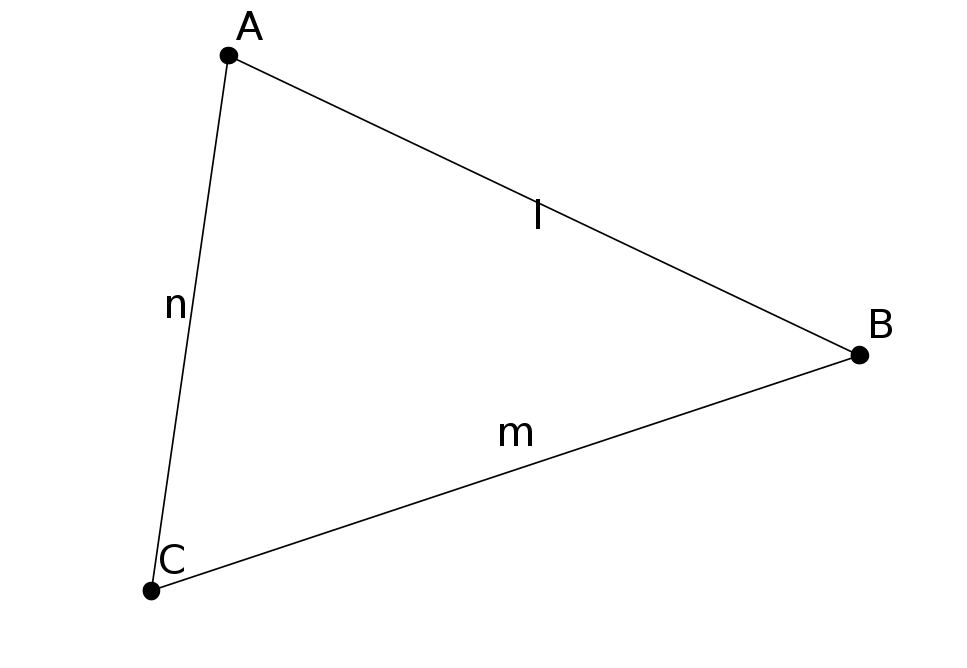
\includegraphics[width=8cm, height=6cm]{images/3pointincidence}
	\caption{Example of incidence geometry $\{l,m,n\}$.}
	\label{fig:incidence1}
\end{figure}

As we can visualize in \ref{fig:incidence1}, $\{l,m,n\}$ is a model of an incidence geometry. Of course, this is not the only model of these axioms. We can use four points, and have six lines with the same result. From \ref{fig:incidence2}, we can see clearly that we can have a model with four points which satisfies the incidence axioms. 

\begin{figure}[H]
	\centering
	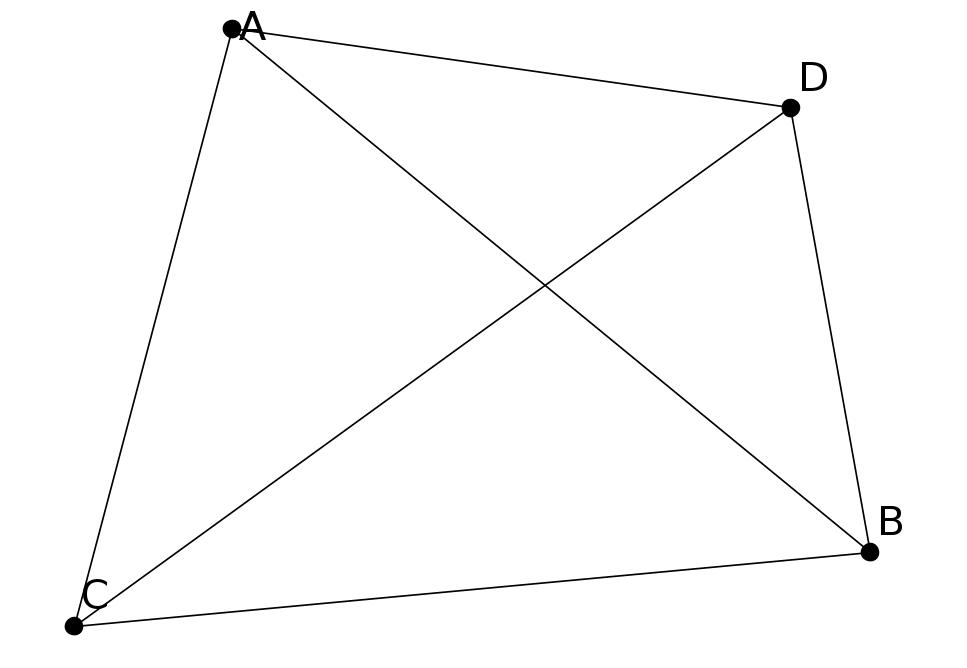
\includegraphics[width=8cm, height=6cm]{images/4pointincidence-a}
	\caption{One model of a four point incidence geometry.}
	\label{fig:incidence2}
\end{figure}

If the fact that two lines `intersecting' in the plane disturbs you, then simply move point $D$ to the located described below. These two models are no different from each other as we shall see later.

\begin{figure}[H]
	\centering
	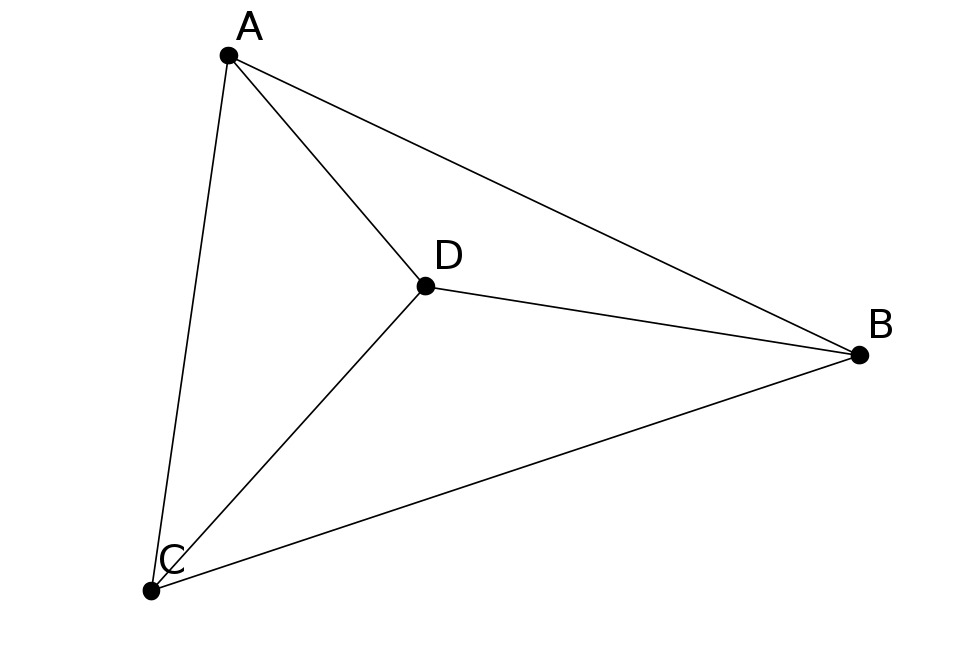
\includegraphics[width=8cm, height=6cm]{images/4pointincidence-a-2}
	\caption{A model of a four point incidence geometry without intersecting lines.}
\end{figure}

Of course, our axioms permit lines containing more than two points since the second axiom states that every line must contain at least two points. So what about a geometry which has a line with three points? Is that even possible given our axioms?  Well consider the geometry with $\mathscr{P}=\{A,B,C,D\}$ in which we have lines $l_1=\{A,B,C\}$, $l_2=\{A,D\}$, $l_3=\{B,D\}$, and $l_4=\{C,D\}$. Notice that this is also a model of an incidence geometry since between every two points there is a unique line containing them, each line has at least two points, and $D\notin l_1$. A visual model of the three point line model is described in figure \ref{fig:incidence3}.


\begin{figure}[H]
	\centering
	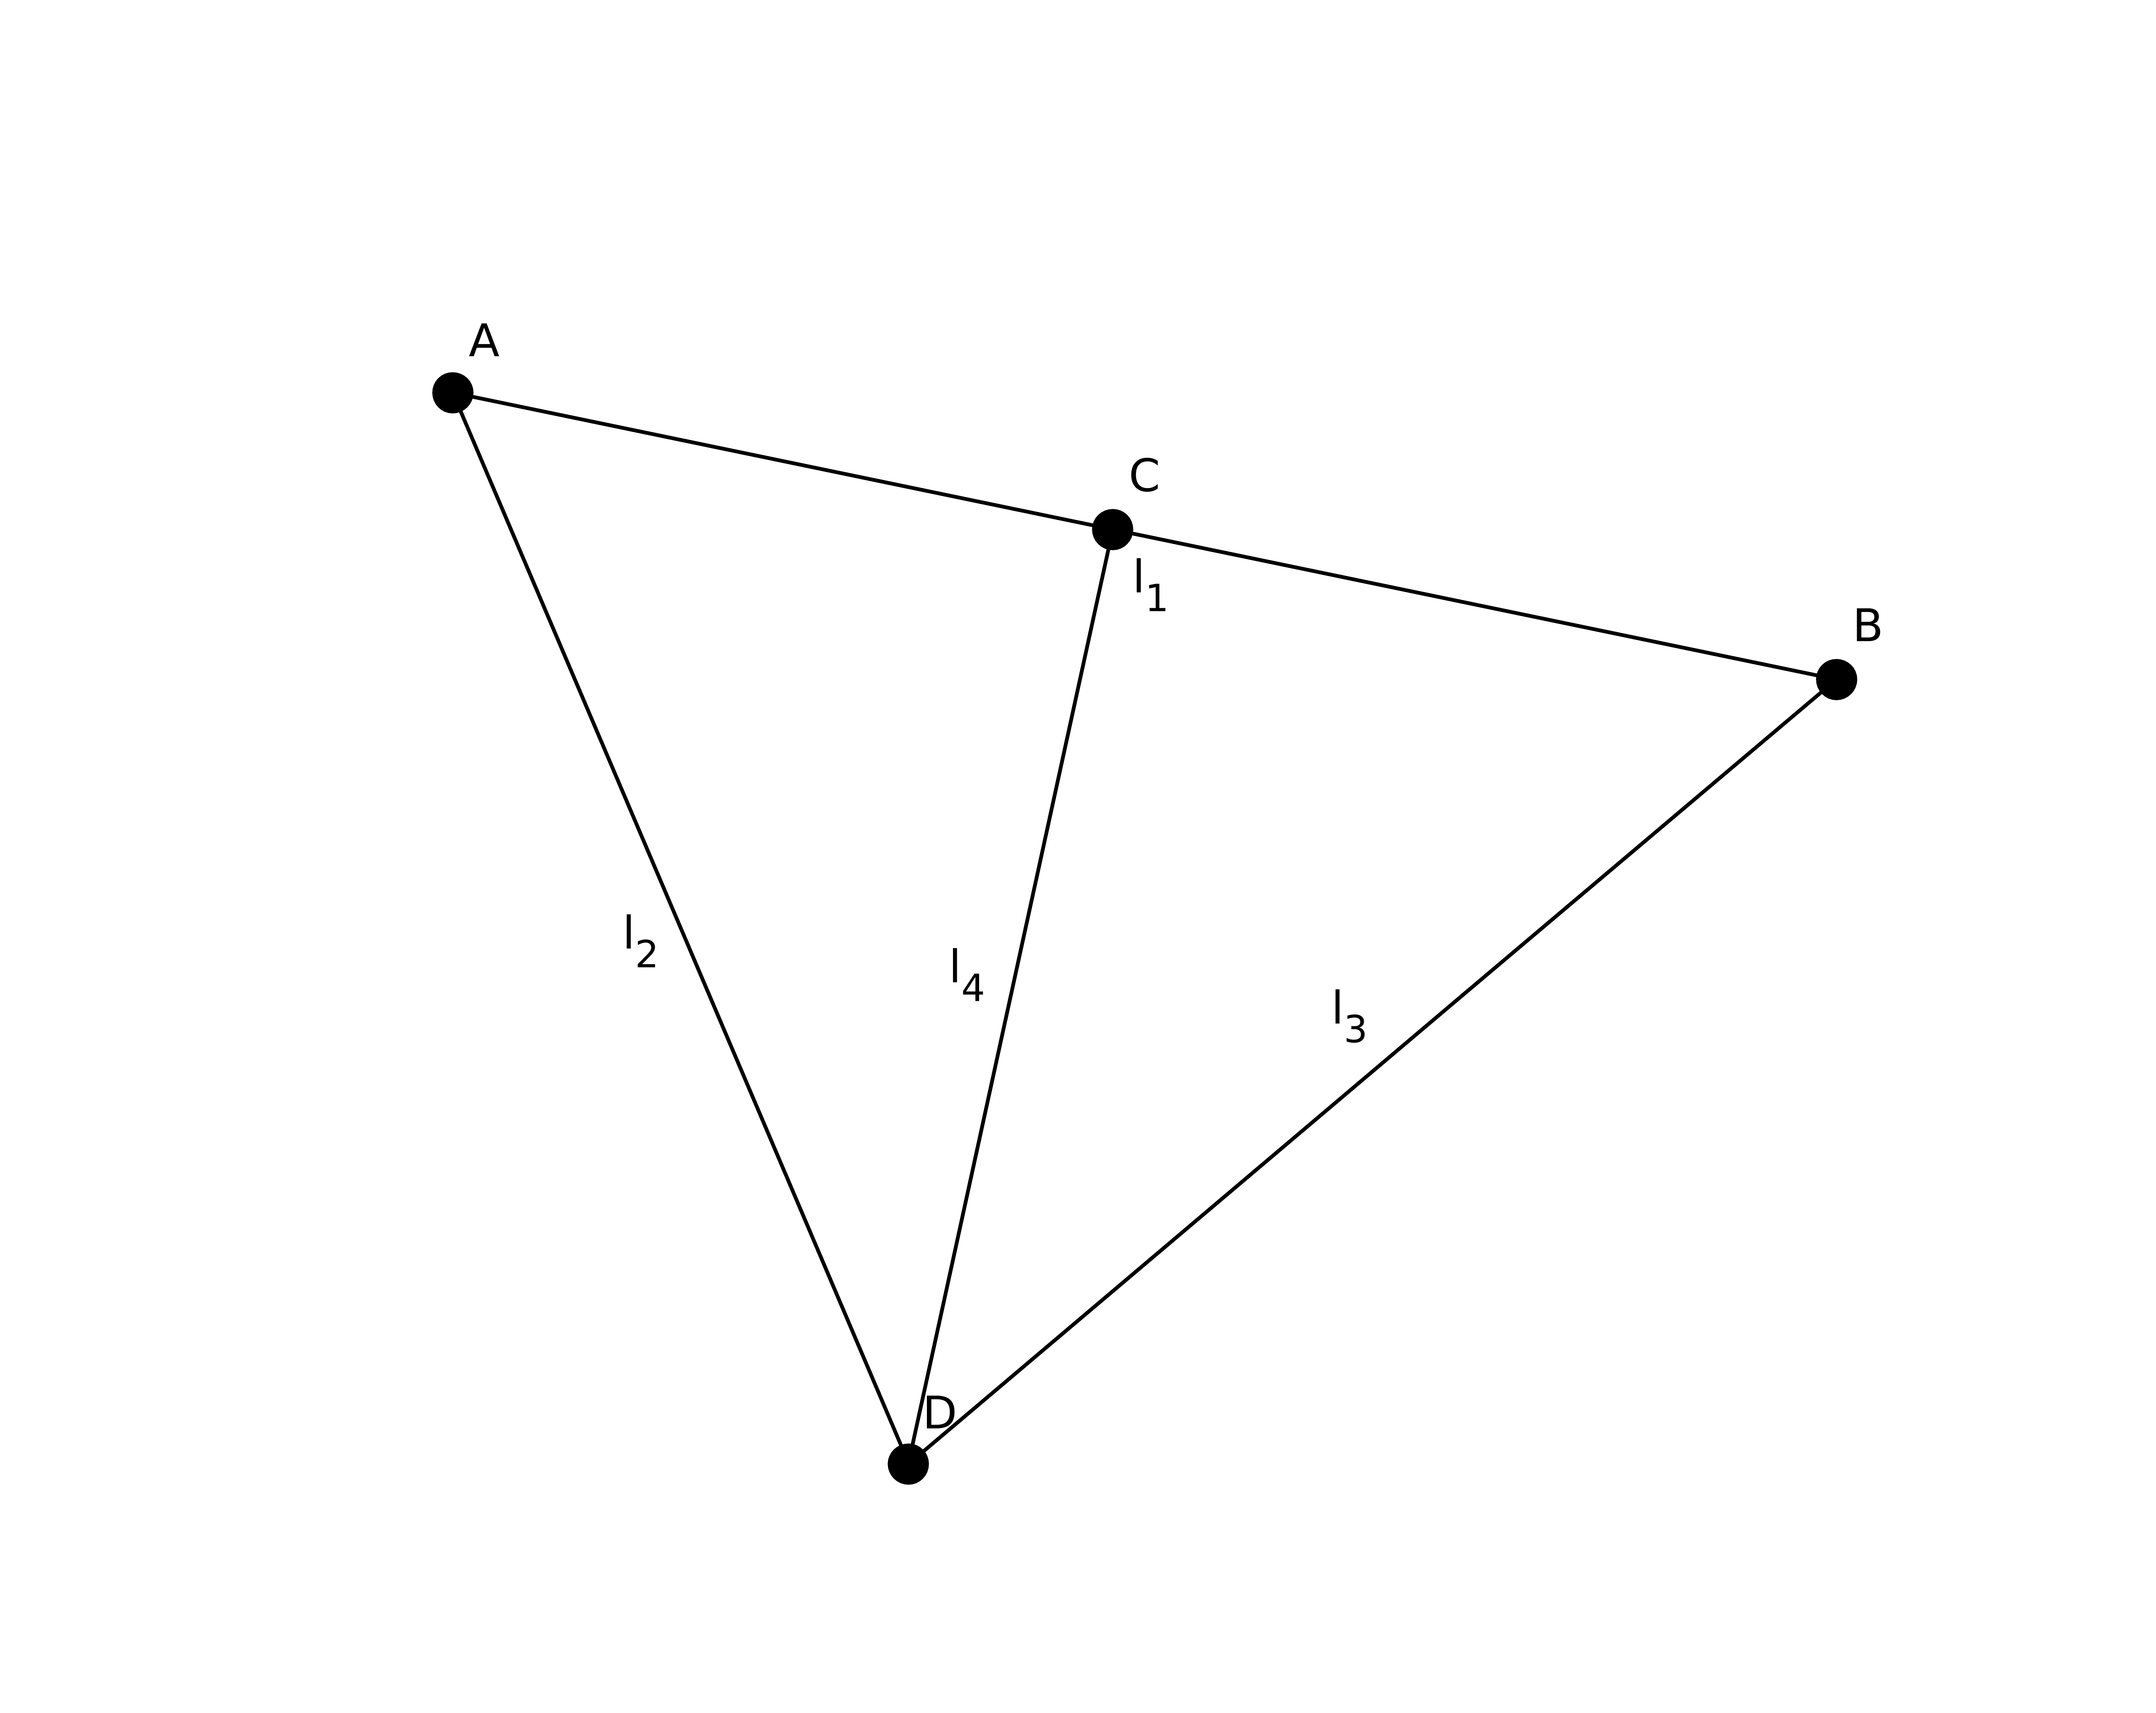
\includegraphics[width=8cm, height=6cm]{images/4pointincidence-b}
	\caption{Another model of a four point incidence geometry. Notice that $l_1$ contains points $A,B,C$ but not $D$.}
	\label{fig:incidence3}
\end{figure}

In general, we say $\Gamma$, a set of axioms, is \textit{satisfiable} whenever we have a model which satisfies all the axioms of $\Gamma$; in other words makes all the axioms true. A \textit{model}, as we saw above, is simply a interpretation of the undefined terms, points and lines, along with a construction or some subset of a desired \textit{universe}, the set we are working within. In the above cases, our universe is points and lines, our constructions or models are \ref{fig:incidence1}, \ref{fig:incidence2}, and \ref{fig:incidence3}, and $\Gamma$ is the set of incidence axioms (i)-(iii). 

Once we have a model which satisfies the incidence axioms, a natural question to ask is what propositions and theorems we can deduce provided this model. For example, we can conclude that the three-point geometry has three lines. We call such a conclusion, a theorem of an incidence geometry, or generally, a theorem of $\Gamma$ if $\Gamma$ is a set of axioms. Now we provide a formal definition of a model.\\

\header{(3.1.1) Definition.} Let $\Gamma$ be a set of axioms. A model of $\Gamma$ is an assignment of interpretations to undefined terms in order to establish verity of the axioms of $\Gamma$.\\

Recall that we mentioned earlier that lines and points were undefined terms. In each model indicated above, we interpreted points to be elements of a set of points and lines to be subsets of the set of points. Once we established these interpretations, we molded these interpretations into constructions to fit the axioms and thus make the axioms true in said model. 

\section{Consistency}
	A natural question to ask at this point is if there is a model of the incidence axioms in which we have a contradiction, that is we are able to show that we can deduce a theorem and its negation. Formally we say the following.\\
	
\header{(3.2.1) Definition.} Let $\Gamma$ be a set of axioms. We say $\Gamma$ is \textit{inconsistent} of there is a theorem in which $\Gamma$ can deduce both the theorem and its negation. We say $\Gamma$ is \textit{consistent} if no such theorem exists.\\
	
Consistency of a set of axioms is a very desirable property because we then know that any theorem we prove will with said set of axioms will never result in a contradiction. This is especially helpful whenever we deal with large bodies of theory like the real numbers or the theory of linear algebra. We want to ensure that such theories are consistent so that they are believable; otherwise we are dealing with empty and useless theories. Unfortunately, it is impossible to demonstrate that a given set of axioms $\Gamma$ is consistent as shown by Kurt G{\"o}del in his \textit{Second Incompleteness Theorem}. Therefore we settle for a weaker property known as \textit{relative consistency}.\\

\header{(3.2.2) Definition.} Let $\Gamma$ be a set of axioms, and let $\Gamma\subseteq\Gamma'$ be an extension of $\Gamma$. We say that $\Gamma$ is \textit{relatively consistent} if and only if $\Gamma'$ has a model.\\

In other words, if there is a model $M$ for some set of axioms $\Gamma'$ for which the set of axioms $\Gamma$ we are trying to prove is consistent is embedded within ($\Gamma\subseteq\Gamma'$), then it is possible to show that the set of axioms is consistent. However, this secretly implies that every it is sufficient to find a model of a set of axioms in order to demonstrate consistency. Note that models are themselves consistent, so we leverage that fact to show that a set of axioms is consistent. Here is a rough sketch of a proof as to why models can show that a set of axioms is consistent is the case.\\

\begin{proofsketch}	
Let $\Gamma$ be a set of axioms which has a model $\cM$. Suppose that $\Gamma$ is inconsistent; fix a theorem $P$ for which $\Gamma$ demonstrates $P$ is true as well as its negation is true. Since $\Gamma$ implies both $P$ and its negation, it must follow that $\cM$ implies both $P$ and its negation, which is a contradiction since any model is consistent. Therefore we must have that $\Gamma$ is consistent.
\end{proofsketch}

\section{Independence}

Now that we have techniques to show whether a set of axioms is consistent, another question arises: do we need all these axioms or can we prove one of the axioms provided the others are true in some model. This brings up the important concept known as \textit{independence}.\\

\header{(3.3.1) Definition.} Let $\Gamma$ be a set of axioms and let $P\in\Gamma$ be an axiom. We say that $P$ is \textit{independent} if we cannot prove $P$ with a model of $\Gamma\backslash\{P\}$. Further, we say $\Gamma$ is \textit{independent} if every $P\in\Gamma$ is independent. Recall that $\Gamma\backslash\{P\}$ means to take $\Gamma$ and exclude the axiom $P$ from $\Gamma$.\\

Independence is useful because it allows us to work in axiom systems that use as few assumptions as possible. Of course, it is more difficult to work in a model in which every axiom is independent since every assumption we previously maintained must now be proved, excluding the axioms themselves, but this is part of the price we pay for elegance. Let us return to the incidence geometry axioms (i)-(iii) and add an additional axiom known as Playfair's axiom. \\

\header{(3.3.2) Axiom.} (Playfair's Axiom) For each point $A$ and each line $l$, there is at most one line containing $A$ which is \textit{parallel} to $l$. We shall denote Playfair's axiom by (P).\\

Note that we used the term \textit{parallel} in this axiom; all parallel means is that if $l$ and $m$ are two lines, then they are parallel if and only if they share no points in common. Now in this example, our goal is to show that each of the axioms are independent from one another. One technique to demonstrate an axioms independence is to find a model of a set of axioms which demonstrates the negation of that axiom while maintaining all the other axioms as true. If this is confusing, what I mean should become clear in the examples below. Let $\Gamma$ be the set of axioms (i)-(iii) together with (P). 

\begin{itemize}
\item First let us prove that we can find a model of $\Gamma\backslash\{(i)\}$ which negates (i). To do this, consider three points in the plane with no lines. Since (i) says that every pair of two distinct points has a unique line, we've successfully negated (i). Now since there are no lines in this model, (ii) is satisfied vacuously. (iii) and (P) follow quickly from the fact that we have no lines as well. Therefore (i) is independent of the other axioms.

\item 
	\parbox[t]{\dimexpr\textwidth-\leftmargin}{%
      \vspace{-2.5mm}
      \begin{wrapfigure}[8]{R}{0.3\textwidth}
        \centering
        \vspace{-\baselineskip}
        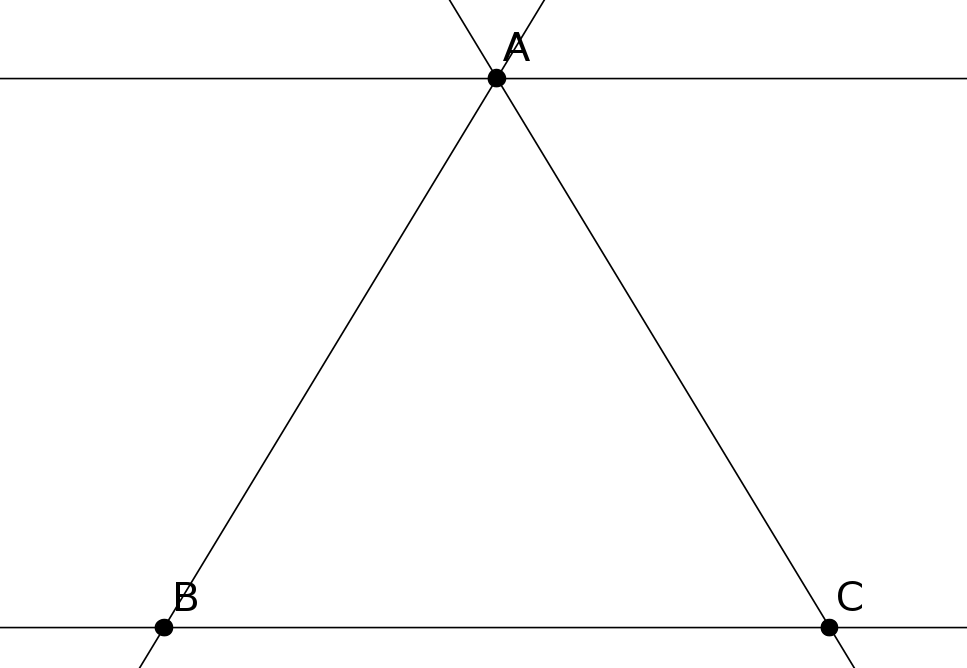
\includegraphics[width=\linewidth]{images/i2independence.png}
      \end{wrapfigure}
      Next let us demonstrate that (ii) is independent. Consider a set of three points $\cP=\{A,B,C\}$ and let lines be the subsets $\{A,B\},\{A,C\},\{B,C\},\{A\}$. Notice that we have satisfied (i) since every two distinct points has a unique line which contains them. We've contradicted (ii) since $\{A\}$ is a line in this model. We've satisfied (iii) since there is no line containing all $A,B,C$. What about (P)? (P) is tricky in this instance. Notice that $\{A,B\}$ and $\{A,C\}$ has no lines containing $C$ and $B$ which are parallel to one another. Also notice that the line $A\notin\{B,C\}$, but $\{A\}$ is a line parallel to $\{B,C\}$ which contains the point $\{A\}$. Therefore we've satisfied (P). Hence (ii) is independent.
    }

\item To show that (iii) is independent, simply consider a two points $\cP=\{A,B\}$ and a line $\{A,B\}$. Notice that (i) is satisfied since points $A$ and $B$ are contained on a unique line, the line $\{A,B\}$ contains at least two points, there are no three noncollinear points, and (P) is satisfied vacuously. Therefore (iii) is independent.

\item 
	\parbox[t]{\dimexpr\textwidth-\leftmargin}{%
      \vspace{-2.5mm}
      \begin{wrapfigure}[7]{R}{0.3\textwidth}
        \centering
        \vspace{-\baselineskip}
        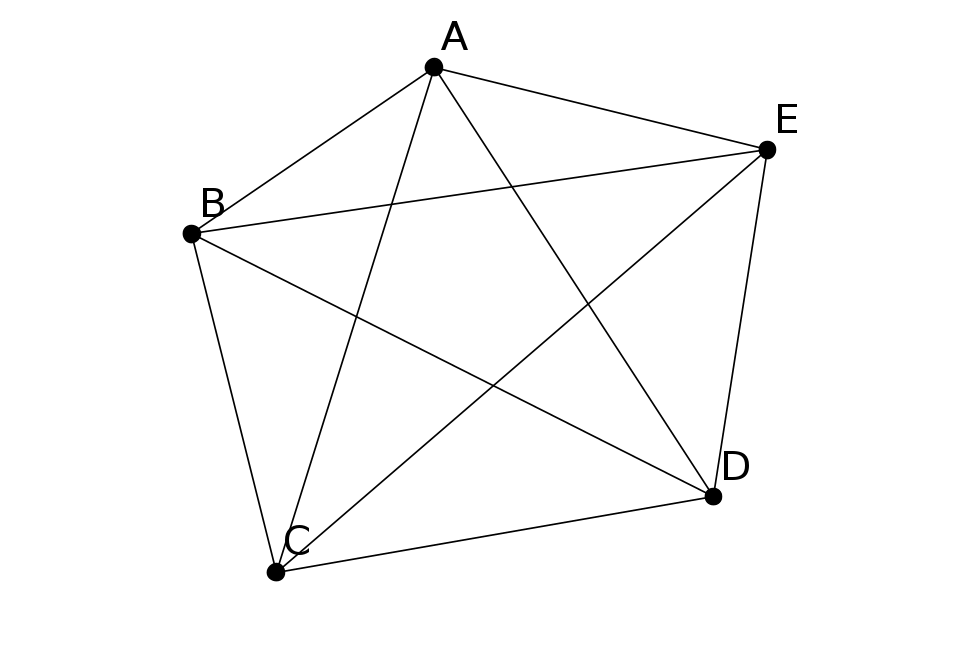
\includegraphics[width=\linewidth]{images/P-independence.png}
      \end{wrapfigure}
	Last, we demonstrate that (P) is independent of (i)-(iii). Consider five points $\cP=\{A,B,C,D,E\}$ and let the lines of this model be every two element subset of $\cP$. Notice that $C$ is not on the line $\{A,B\}$, but there are two lines $\{C,E\}$ and $\{C,D\}$ which contain $C$ and are parallel to $\{A,B\}$. Hence (P) is false in this model. For the other axioms, notice that every set of two points has a unique line between them, every line contains two points by hypothesis, and $A,B,C$ are three noncollinear points. Thus (P) is independent of (i)-(iii).
    }
\end{itemize}

Note that above we required four distinct models to show that all four axioms were independent of one another. In general, we require for there to be $n$ distinct models to show that $n$ axioms are independent. Of course, we can then ask the question: how do we know that there are $n$ distinct models? Could we have two models of an incidence geometry that `look the same'? This brings up the idea known as isomorphisms, which we will now discuss.

\section{Isomorphisms and Completeness}

\header{(3.4.1) Definition.} Let $\Gamma$ be a set of axioms and let $\cM$ and $\cN$ be models of $\Gamma$. We say that $\cM$ and $\cN$ are \textit{isomorphic} if and only if there exists a bijection $\varphi\colon\cM\rightarrow\cN$ with the property that each point is mapped to a unique point, each line is mapped to a unique line, and preserves all relations. In particular if $P$ and $l$ are a point and line in $\cM$ respectively, then $\varphi(P)$ and $\varphi(l)$ are a point and line in $\cN$ respectively. If $\varphi$ exists, then we say that $\varphi$ is an \textit{isomorphism}.\\

	Isomorphisms are a mouthful; let's break this definition down. Let $\cM$ be the model described in figure \ref{fig:incidence2} and $\cN$ be the model described in figure \ref{fig:incidence3}. Recall from Linear Algebra that a bijection is a function which is one-to-one and onto (injective and surjective). Therefore, we must have some mapping between $\cM$ and $\cN$ which maps each point and line of $\cM$ to a unique point and line of $\cN$ respectively. If $\cM$ and $\cN$ are isomorphic models, then $\cM$ and $\cN$ have some bijection between the set of their sets of points. 

	In both models $\cM$ and $\cN$, we have a four point model, so such a bijection could exist; let's suppose it's the identity mapping, that is if $\varphi$ is our isomorphism, $\varphi(A)=A$ for all points $A$ in the model $\cM$. Further, we need a mapping which sends lines to lines, that is if $l$ is a line in the model $\cM$, $\varphi(l)$ must also be a line in $\cM$. However, notice that $\cN$ has four lines, and $\cM$ has six lines. Therefore we cannot have a bijection between the set of lines of $\cM$ and $\cN$ which contradicts the fact that we had an isomorphism between $\cM$ and $\cN$. Therefore we must conclude that $\cM$ and $\cN$ are not isomorphic. From this conclusion, we may say that there are two distinct models of a four point incidence geometry. As it turns out, those are the only two models of an incidence geometry with four points that are possible -- we leave this as an exercise to show. 
	
	In particular when we have an isomorphism between two models, isomorphisms also preserve the relation on the sets, that is if $a\sim b$ in $\cM$, $\varphi(a)\sim\varphi(b)$ as well. To demonstrate when this could go wrong, consider the following example. Let $\cM$ and $\cN$ be models of the real line $\R$ with an additional point $x\notin\R$ so that $\cM$ and $\cN$ are models of an incidence geometry. Consider $\R$ under the betweenness relation described earlier. Fix points $A,B,C\in\R$ with $A<B<C$. Then the mapping $\varphi\colon\R\rightarrow\R$ defined as
	\[\varphi(P)=\begin{cases}
	P & \text{if } P\notin\{B,C\}\\
	C & \text{if } P=B\\
	B & \text{if } P=C\\
	\end{cases}\]  
is not an isomorphism of between $\cM$ and $\cN$ despite the fact that it is a bijection which sends all points uniquely to points and all lines uniquely to lines. The reason it fails is because it does not preserve the betweenness relation on $\R$ which is required in the definition of an isomorphism. 

	Let $\Gamma$ be the set of the incidence geometry axioms together with a new axiom: \textit{There are exactly three distinct points.} Notice that figure \ref{fig:incidence1} is a model of $\Gamma$. Let figure \ref{fig:incidence1} be the model $\cM$. Now if $\cN$ is any other model of $\Gamma$, it turns out that $\cM$ and $\cN$ are isomorphic to one another. To see this, let $\cP=\{1,2,3\}$ be the set of points of $\cN$. By (iii), there is no line containing all three points. By (i), we must have at least three lines, $\{1,2\}$, $\{1,3\}$, $\{2,3\}$, and these are all the lines by (ii). Hence all lines of $\cN$ are two point subsets of $\cP$. Notice that $\cM$ has the same property, that is all its lines are two element subsets of its points. Therefore since there are no relations, $\cM$ and $\cN$ are isomorphic. Since $\cN$ was any other model, we conclude that all models of $\Gamma$ are isomorphic to one another. 
	
	Since $\Gamma$ has this property that all models of $\Gamma$ are isomorphic to one another, we say $\Gamma$ is \textit{categorical}, that is there is a unique model of this particular set of axioms. We say that $\cM$, a model of $\Gamma$ is then unique up to isomorphism. What the phrase \textit{unique up to isomorphism} means is that we have one and only one model that is distinct between isomorphisms. 
	
	Furthermore, let $\psi$ be an arbitrary theorem deducible from $\Gamma$. We say that $\Gamma$ is \textit{complete} whenever we can deduce that $\psi$ is true or the negation of $\psi$ is true. In general, it is impossible to demonstrate that a system is complete. However, there are specific conditions, that when met, allow us to conclude that $\Gamma$ is complete. One such condition is when all models of $\Gamma$ are isomorphic to one another.
	
\subsection*{Exercises}
\begin{enumerate}
\item Let $\Gamma$ be the set of incidence geometry axioms with an additional axiom: \textit{There are exactly five distinct points.}
\begin{enumerate}
	\item Show that $\Gamma$ is consistent.
	\item Show that $\Gamma$ is independent.
	\item Prove or disprove the following statements:
	\begin{enumerate}
		\item Every line contains exactly two points.
		\item Every pair of lines meets at exactly one point.
	\end{enumerate}
	\item Show that there exist two distinct models which are not isomorphic.
	\item Is $\Gamma$ complete? Why or why not?
\end{enumerate}
\item An \textit{automorphism} is an isomorphism on a model $\cM$ which is in 1-to-1 correspondence with itself. How many distinct automorphisms does the three point incidence geometry have?
\item An \textit{affine plane} is a set of points and subsets called lines satisfying (i), (ii), (iii), and a stronger version of Playfair's Axiom.

\noindent \textbf{P`.} For every line $l$ and every point $A$, there exists a unique line $m$ containing $A$ and parallel to $l$. 

Demonstrate the following.
\begin{enumerate}
	\item Show that any two lines in the affine plane have the same number of points, that is if line $l$ has $m$ points and line $k$ has $n$ points, then $m=n$.
	\item Show that if an affine plane has a line with exactly $n$ points, then the total number of points in the plane is $n^2$.
	\item Show that the real Cartesian plane is an affine plane. (\textit{Hint:} Show that $\R^2$ satisfies all the axioms of an incidence geometry and \textbf{P`}.)
\end{enumerate}
\item Show the converse of the condition for completeness described in the end of this section is false, that is show \textit{if $\Gamma$ is complete, then all models of $\Gamma$ are isomorphic to one another} is false.
\item In a finite incidence geometry, show that the number of lines is greater than the number of points. (\textit{Hint:} Proceed by induction on the number of points.)
\end{enumerate}
	

\vfill
\pagebreak

\chapter{Euclid's Geometry}
\section{Euclid's Postulates and Definitions}
\section{Proposition 1, 2, 4, and 8}
\section{Proposition 9, 10, 11, and 12}

\chapter{Linear Algebra Review}

	This chapter will review Linear Algebra from its basic constructions of vector spaces to linear transformations of vector spaces and their respective eigenspaces. This review will give us some key insights into the core of geometric transformations of the Euclidean plane in preparation for Chapter 3. 

	Recall that a vector space is a mathematical structure which couples a set of vectors with a field of scalars in $\R$. In the previous course on Linear Algebra, we explored vectors in the plane; we will generalize to vectors in $\R^3$ where the vectors are now in Euclidean plane oriented in $\R^3$. We will also slightly generalize the notion of a field of scalars to arbitrary fields, though we will continue to work on $\R$. Within each vector space, we had two operations, vector sums, which took two vectors $x,y$ in the set of vectors and returned a new vector $x+y$, and scalar multiplication, which allowed these these vectors to interact with field of scalars by 'scaling' a vector. 

\section{Vector Spaces}

Fields are special algebraic structures which mimic the algebraic properties of $\R$. A field has two operations, addition and multiplication, and these operations are \textit{closed}, that is they return an element of the field they operate over. Addition as a function is defined as you would expect, $+\colon\R\rightarrow\R$ such that $+(x,y)=x+y$ and similarly with multiplication $\cdot\colon\R\rightarrow\R$ such that $\cdot(x,y)=x\cdot y$. In order to for a field to mimic the algebraic properties of $\R$ we state some necessary assumptions about the field which we will call $\cF$.\\

\noindent\textbf{(5.1.1) Definition.} A \textit{field} is an algebraic structure with two operations which obeys the following axioms.
\begin{enumerate}[itemsep=0.1cm]
\item $+$ is \textit{associative}, that is for all $x,y,z\in\cF$, $(x+y)+z=x+(y+z)$.
\item $+$ is \textit{commutative}, that is for all $x,y\in\cF$, $x+y+y=y+x$.
\item $\cF$ has an \textit{additive identity}, that is for all $x\in\cF$, there exists $\eq[0]\in\cF$ such that $x+\eq[0]=x=\eq[0]+x$.
\item $\cF$ has \textit{additive inverses}, that is for all $x\in\cF$, there exists $y\in\cF$ such that $x+y=\eq[0]=y+x$.
\item $\cF$ has a \textit{distributive property}, that is for all $w,x,y,z\in\cF$, \[(x+y)\cdot(w+z)=x\cdot w+x\cdot z+y\cdot w+y\cdot z.\]
\item $\cdot$ is \textit{associative}, that is for all $x,y,z\in\cF$, $(x\cdot y)\cdot z=x\cdot(y\cdot z)$.
\item $\cdot$ is \textit{commutative}, that is for all $x,y\in\cF$, $x\cdot y=y\cdot x$.
\item $\cF$ has a \textit{multiplicative identity}, that is for all $x\in\cF$, there exists $\eq[1]\in\cF$ such that $x\cdot \eq[1]=x=\eq[1]\cdot x$.
\item $\cF$ has \textit{multiplicative inverses}, that is for all $x\in\cF$, there exists $y\in\cF$ such that $x\cdot y=\eq[1]=y\cdot x$.
\end{enumerate}

Because we are assuming specific algebraic properties of the real numbers, we can demonstrate that a vector space, with its axioms, are provable from the real numbers and the operations of vector sums and scalar multiplication. Because of a field's properties, we can show that the identities in a field are unique, the inverses of a field are unique, and elements of the field under the operations associate in general. From these principles, we define a vector sums and scalar multiplication. Recall that we may write vectors as $n$-tuples. In this case, we will use ordered triples to represent vectors in 3-space. Scalars will just be elements of $\cF$. In short, we will write $V$ is a set over a field $\cF$ to mean that $x\in V$ has entries in $\cF$.\\

\noindent\textbf{(5.1.2) Definition.} Let $V$ be a set of vectors and $\cF$ be a field of scalars.
\begin{enumerate}
\item For vectors $x,y\in V$ with $x=(x_1,x_2,x_3)$ and $y=(y_1,y_2,y_3)$, we define the vector sum to be a function $+\colon V\times V\rightarrow V$ such that 
\[x+y=(x_1,x_2,x_3)+(y_1,y_2,y_3)=(x_1+y_1,x_2+y_2,x_3+y_3).\]
\item For any vector $x\in V$ and scalar $k\in\cF$, we define scalar multiplication to be a function $\cdot\colon\cF\times V\rightarrow V$ such that
\[\cdot(k,x)=k\cdot x=k(x_1,x_2,x_3)=(k\cdot x_1,k\cdot x_2,k\cdot x_3).\]
\end{enumerate}

We will simply write $x+y$ and $k\cdot x$ to stand for vector sums and scalar multiplication respectively since the function notation is cumbersome.\\

\noindent\textbf{(5.1.3) Example.} Let $V=\R^3$ and $K=\R$. Then the set of vectors are ordered triples with entries in $\R$, ascertaining the algebraic properties for each operation from the fact that $\R$ is a field. For example, let $x,y\in V$ with $x=(x_1,x_2,x_3)$ and $y=(y_1,y_2,y_3)$, then we may show that $x+y$ commute as follows.
\begin{align*}
x+y & = (x_1,x_2,x_3) + (y_1,y_2,y_3)\\
 & = (x_1+y_1,x_2+y_2,x_3+y_3) & \text{(definition of vector sum)}\\
 & = (y_1+x_1,y_2+x_2,y_3+x_3) & \text{(by commutative properties of $\cF$)}\\
 & = (y_1,y_2,y_3) + (x_1,x_2,x_3) & \text{(definition of vector sum)}\\
 & = y+x
\end{align*}

\noindent\textbf{(5.1.4) Notation.} From hereon, when we write a vector with its entries, we will write vectors explicitly in their column form, if $V$ is a vector space and $x\in V$, then 
\[x=\begin{pmatrix}
x_1\\
x_2\\
x_3
\end{pmatrix},\]
where $x_i\in\cF$ for all $i\in\{1,2,3\}$. We will also write $kx$ to mean $k\cdot x$.

From these two definitions, it's possible to show that vector sums are associative, commutative, and scalar multiplication is associative and commutative by levering the properties of the field in which the entries of the vector and scalars are contained in. It's also possible to show that from the fact that $0,1\in\cF$ that vector sums have an identity as well as scalar multiplication. Furthermore, vector sums then have additive inverses, and together the two operations have a distributive property. From this point, we may define a vector space $V$ over a field $\cF$.\\

% Vector Spaces

\noindent\textbf{(5.1.5) Definition.} A \textit{vector space} over a field $\cF$ is a set $V$ together with vector sums and scalar multiplication given in \textbf{(5.1.2)} which obey the following axioms:
\begin{enumerate}[label=\arabic*), itemsep=0.7mm]
\item For all $x,y,z\in V$, $(x+y)+z=x+(y+z)$.
\item For all $x,y\in V$, $x+y=y+x$.
\item There exists $\eq[0]\in V$ such that for all $x\in V$, $x+\eq[0]=x$.
\item For each $x\in V$, there exists a vector $y\in V$ such that $x+y=\eq[0]$.
\item For all vectors $x,y\in V$ and all scalars $c\in\cF$, $c(x+y)=cx+cy$.
\item For all vectors $x\in V$ and all scalars $c,d\in\cF$, $(c+d)x=cx+dx$.
\item For all vectors $x\in V$ and for all scalars $c,d\in\cF$, $c(dx)=(cd)x$.
\item For all vectors $x\in V$, there exists $\eq[1]\in\cF$ such that $\eq[1]x=x$.
\end{enumerate}

From hereon, we will call the identity of a vector space the zero vector and denote it with $\vec{0}$. Just as in the case of a field, its possible to show that the identity of a vector space is unique, that vectors have unique inverses, and the zero scalar times any vector is the zero vector.

\vfill
\pagebreak

\noindent\textbf{(5.1.6) Proposition.} Let $V$ be a vector space over a field $\cF$.
\begin{enumerate}
\item For all $x,y,z$ if $x+y=x+z$, then $y=z$. 
\item For all $x\in V$, $0x=\vec{0}$.
\item For all $x\in V$ and $c\in\cF$, $(-c)x=-(cx)$.
\end{enumerate}

\begin{enumerate}
\item\begin{proof} Let $x,y,z\in V$ be arbitrary with $x+y=x+z$. Since $x\in V$, $-x\in V$ exists, so add $-x$ to $x+y=x+z$ to the left on both sides to obtain 
\begin{align*}
x+y=x+z & \Leftrightarrow (-x)+(x+y)=(-x)+(x+z) & \text{(introducing additive identity)}\\
 & \Leftrightarrow(-x+x)+y=(-x+x)+z & \text{(addition is associative)}\\
 & \Leftrightarrow \vec{0}+y=\vec{0}+z & \text{(application of additive inverses)}\\
 & \Leftrightarrow y=z & \text{(application of axiom 3)}
\end{align*}
\end{proof}
\item\begin{proof}
Let $x\in V$ be arbitrary. Notice the following
\begin{align*}
0x & = (0+0)x & \text{(application of axiom 3)}\\
 & = 0x+0x & \text{(application of axiom 6)}\\
 & \Leftrightarrow 0x-0x=(0x+0x)-0x & \text{(introducing additive inverse)}\\
 & \Leftrightarrow \vec{0} = 0x & \text{(applying additive inverses)}
\end{align*} 
\end{proof}
\item\begin{proof}
Let $x\in V$ and $c\in\cF$ be arbitrary. Consider the expression $cx+(-c)x$. Notice by axiom 6 that $cx+(-c)x=(c+-c)x=0x=\vec{0}$. Hence $cx+(-c)x=\vec{0}$ or in other words $-(cx)+cx+(-c)x=-(cx)$ if and only if $-(cx)=(-c)x$.
\end{proof}
\end{enumerate}

% Subspaces

\noindent\textbf{(5.1.7) Definition.} Let $V$ be a vector space. We say $W\subseteq V$ is a subspace of $V$ if and only if $W$ is a vector space under the operations of vector sum and scalar multiplication from $V$.\\

\noindent\textbf{(5.1.8) Proposition.} Let $V$ be a vector space and $W\subseteq V$ be a subset. $W$ is a subspace of $V$ if and only if for all $x,y\in W$ and $c\in\cF$, we have $cx+y\in W$.

\begin{proof}
We prove the forward direction and leave the reverse as an exercise. Suppose $W$ is a subspace of $V$. Then for all $x\in W$, we have $cx\in W$ and for all $y\in W$, we have $cx+y\in W$ because $W$ is closed under vector sums and scalar multiplication.
\end{proof}

% do example involving lines and planes

% intersect planes to make lines.

% intersect lines to make points and make a point

% Span

\noindent\textbf{(5.1.10) Definition.} Let $V$ be a vector space over a field $\cF$. Let $S\subseteq V$ be a subset of $V$.
\begin{enumerate}[label=(\alph*)]
\item A \textit{linear combination} of vectors in $S$ is any sum $a_1x_1+a_2x_2+\cdots+a_nx_n$ where $a_i\in\cF$ and $x_i\in S$ for all $i$
\item The set of all linear combinations of a set $S$ is called the \textit{span} of $S$ and is denoted $Span(S)$. If $S=\emptyset$, then $Span(S)=\{\vec{0}\}$. Lexically, if $W\subseteq V$ is any subset, then we say that $S$ \textit{spans} or \textit{generates} $W$. 
\end{enumerate}

% Linear Dependence
\noindent\textbf{(5.1.11) Definition.} Let $V$ be a vector space over a field $\cF$, and let $S\subseteq V$ be a subset of $V$.
\begin{enumerate}[label=(\alph*)]
\item $S$ is a linearly dependent set if there exists a finite number of vectors $x_i$ and coefficients $a_i$ not all zero such that $a_1x_1+a_2x_2+\cdots+a_nx_n=\vec{0}$.
\item $S$ is a linearly independent set if whenever we have $a_i\in\cF$ and $x\in S$ such that $a_1x_1+a_2x_2+\cdots+a_nx_n=\vec{0}$, then $a_i=0$ for all $i$. In other words, $S$ is linearly independent when it is not linearly dependent.
\end{enumerate}

% Basis and Dimension

\noindent\textbf{(5.1.12) Definition.} A subset $S$ of a vector space $V$ is called a \textit{basis} of $V$ if $V=Span(S)$ and $S$ is linearly independent.\\

\noindent\textbf{(5.1.13) Definitions.}
\begin{enumerate}[label=(\alph*)]
\item If $V$ is a vector space with some finite basis, we say $V$ is finite-dimensional.
\item Let $V$ be a finite-dimensional vector space. The \textit{dimension} of $V$, denoted $\dim(V)$, is the number of vectors in a basis of $V$. We denote the dimension of $V$ by $\dim(V)$.
\item If $V=\{\vec{0}\}$, we define $\dim(V)=0$.
\end{enumerate}

\subsection*{Exercises}
\begin{enumerate}[itemsep=0.2mm]
\item Let $V$ be a vector space over a field of scalars $\cF$. If $W\subseteq V$ is a subspace, show that $0\in W$.
\item \begin{enumerate}
\item Show that in $V=\R^2$, any line through the origin is a subspace.
\item Show that in $V=\R^3$, any line or plane through the origin is a subspace.
\end{enumerate}
\item Let $V=\R^2$ and $\cF=\R$. Let $W_1$ and $W_2$ be two distinct subspaces of $V$. When is $W_1\cup W_2$ a subspace of $V$? When is $W_1\cap W_2$ a subspace?
\item Let $\{u,v,w\}$ be a linearly independent subset of a vector space. Show that $\{v+w,u+w,v+w\}$ is also linearly independent.
\item Show that if $S$ is a linearly independent subset of a vector space $V$ and $S=\{S_1\cup S_2\}$ with $S_1\cap S_2=\emptyset$, then $Span(S_1)\cap Span(S_2)=\{\vec{0})$.
\item Show that $S=\{(1,1,1)(1,1,0),(1,0,0)\}$ and $S'=\{(1,1,1),(0,1,1),(0,0,1)\}$ are both bases of $\R^3$.
\end{enumerate}

\section{Linear Transformations}

% Linear Transformations

\noindent\textbf{(5.2.1) Definition.} A function $T\colon V\rightarrow W$ is called a linear transformation or linear mapping if 
\begin{enumerate}
\item $T(u+v)=T(u)+T(v)$ for all $u,v\in V$
\item $T(\alpha u)=\alpha T(u)$ for all $u\in V$ and $\alpha\in\cF$.
\end{enumerate}

% Examples of Linear Transformations

% Matrix Representation of a Linear Transformation

% Matrix Addition and Multiplication

% Rank-Nullity

% Matrix Inversion

% Change of Basis

\section{Determinants}

% Definition and Area Principle

% 2x2 Case

% 3x3 Case

% Recursive Definition

\section{Eigenstuff}

% Eigenspaces and Eigenvectors

% Diagonalization of a Matrix

% Orthogonal Spaces

% Gram-Schmidt Orthogonalization


\chapter{Basic Group Theory}

In Chapter 3, Judith discusses and utilizes the notion of a \textit{Group} without going into much detail about what they are. So what exactly is a Group, where do they come from, and why do we care? Groups, as we shall see shortly, are a generalization of many natural properties, such as associativity, of say the integers to an abstract structure. Because many algebraic structures such as matrices and functions exhibit many of the same properties, we naturally abstract with these properties alone to the notion of a group, studying these properties in isolation, and then returning to the domains from whence they came.\\

\header{(6.1.1) Definition.} Let $X$ be a set. We say that a \textit{binary operator} on $X$ is a function $f\colon X\times X\rightarrow X$. \\

In other words, a binary operator is a function which combines two inputs of $X$ to create a new input. One very important note is that if $a,b\in X$ and $f$ is a binary operation on $X$, then $f(a,b)\in X$ by definition of $f$. Now, let's define a group.\\

\header{(6.1.2) Definition.} Let $G$ be a set equipped with a binary operation $\cdot$. We say that $(G,\cdot)$ is a group if it satisfies the following properties:
\begin{itemize}
\item $\cdot$ is associative, that is for all $g_1,g_2,g_3\in G$, we have $(g_1\cdot g_2)\cdot g_3 = g_1\cdot (g_2\cdot g_3)$.
\item $G$ has an identity element, that is there exists $e\in G$ such that for all $g\in G$, we have $e\cdot g=g\cdot e=g$.
\item $G$ has inverses, that is for all $g\in G$, there exists $h\in G$ with $g\cdot h=h\cdot g=e$. When $g$ has a unique inverse, we denote it by $g^{-1}$.
\end{itemize}

You're probably wondering why groups consist of these properties specifically and, not say, commutativity. Well in general, many of the algebraic structures that we care about exhibit all three of these properties. For example in $\Z$ under addition (we'll write it as $(\Z,+)$), $+$ does associate, 0 is an additive identity of $\Z$, and for every $m\in\Z$, simply take the negative of $m$ and add the two together to get to 0. Therefore $(\Z,+)$ is in fact a group under addition. 

As for another example, consider the set of all nonsingular matrices of dimension $n\geq 1$ whose coefficients lie in $\R$. As you may recall from Linear Algebra, matrix multiplication does in fact associate, matrices have an identity under matrix multiplication, and every nonsingular matrix is invertible. We will denote this group by $GL_n(\R)$ or in English, the \textit{General Linear Group over $\R$}.

One thing to note about these two groups is that on the one hand, $+$ on $\Z$ is commutative, while matrix multiplication on $GL_n(\R)$ is not commutative. Recall back from Chapter 3 when we spoke about independence. It's far more elegant and flexible to work with a smaller set of axioms than a large structure. Even though including commutative would add only one additional axiom to the groups, we prefer to go on without it. However, we do have a notion for commutative groups.\\

\header{(6.1.3) Definition.} Let $(G,\cdot)$ be a group. We say that $(G,\cdot)$ is \textit{abelian} if and only if for all $g_1,g_2\in G$, we have that $g_1\cdot g_2=g_2\cdot g_1$. \\

In the above instances, we can say that $(\Z,+)$ is an abelian group while $(GL_n(\R),\cdot)$ is a nonabelian group.

\section{Basic Group Theory}

\header{(6.2.1) Examples.}
Groups are very abstract structures so it's important to understand their examples first. 

\header{(6.2.2) Proposition.} Let $(G,\cdot)$ be a group. Then the following are true.
\begin{enumerate}
\item The identity of $G$ is unique.
\item $g^{-1}$ is uniquely determined.
\item $(g^{-1})^{-1}=g$ for all $g\in G$.
\item $(g_1\cdot g_2)^{-1}=g_2^{-1}\cdot g_1^{-1}$.
\item $\cdot$ associates in general, that is $g_1\cdot g_2\cdot g_3\cdots\cdot g_n$ is the same for all $n\in\N^+$ regardless of how the parentheses are placed.
\end{enumerate}

\section{The Dihedral Group}
\section{The Symmetric Group}
\section{Geometric Transformation Groups}

\end{document}